\documentclass [a4paper, 12pt]{amsbook}

\usepackage{german}
\usepackage[latin1]{inputenc}
\usepackage{graphicx}
\usepackage{amsmath}
\usepackage{amssymb}
\usepackage{pstricks}
\usepackage{eurosym} 			%fr  Symbol
\usepackage{fancyhdr}
%\usepackage{hyperref}

\newtheorem{satz}{Satz}[section]
\newtheorem{beweis}{Beweis}[section]
\newtheorem{definition}{Definition}[section]
\newtheorem{bsp}{Beispiel}[section]

\pagestyle{fancy}% muss vor \renewcommand{\sectionmark} stehen
\fancyhf{}
\fancyhead[R]{\thepage}% gerade Seiten, links
\fancyhead[L]{\leftmark}% gerade Seiten, rechts
%\fancyhead[OL]{\rightmark}% ungerade Seiten, links
%\fancyhead[OR]{\thepage}% ungerade Seiten, rechts
\renewcommand{\sectionmark}[1]{
\markboth{\thesection{} #1}{\thesection{} #1}
}
\renewcommand{\subsectionmark}[1]{
\markright{\thesubsection{} #1}
}

\begin {document}
\title{Leistungskurs Mathematik 12 / 13}
\author{Fabian Nick}

\begin{titlepage}
\begin{center}
\textbf{\LARGE Leistungskurs Mathematik NRW}\\

\today \\

von: Fabian Nick

\begin{figure}[hp]
	\centering
		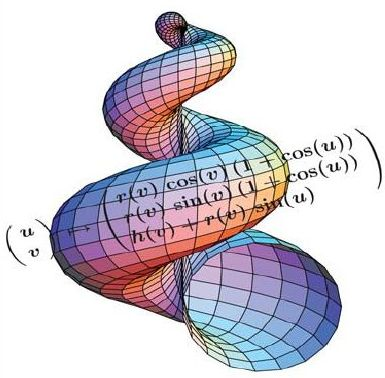
\includegraphics[width=1.0\textwidth]{abbildungen/3dplot.jpg}
	\label{fig:3dplot}
\end{figure}

\end{center}
\end{titlepage}


\textbf{�ber dieses Dokument:}\\
Dieses Dokument beruht auf den Mitschriften aus dem Mathematikunterricht von Frau M. Peters im Leistungskurs des Abiturjahrgangs 2008 am Nicolaus Cusanus Gymnasium Bergisch Gladbach (NRW). Seit dem Abitur im April 2008 wird dieses Dokument st�ndig Verbesserungen und Erweiterungen unterzogen.\\
Dies Aufzeichnungen sind weder vollst�ndig, noch vollst�ndig korrigiert. Es k�nnten also sowohl Rechtschreibfehler als auch \textbf{inhaltliche Fehler} vorhanden sein. Verbesserungsvorschl�ge, Korrekturen etc sind gerne willkommen unter fp.nick@gmail.com\\
\quad\\
Das Themengebiet \textit{Stochastik} fehlt in diesem Skript (noch), da es auch im Unterricht nur angerissen wurde und die Informationen somit recht beschr�nkt sind. Wer Interesse daran hat, zur Vervollst�ndigung dieses Skripts beizutragen, kann sich gerne �ber die unten angegebenen Kontaktdaten bei mir melden. LaTeX Kenntnisse sind dabei in jedem Fall hilfreich!\\
Weiterhin ist auch ein Teil mit �bungsaufgaben zu den einzelnen Kapiteln geplant. Wer hier mitwirken will ist ebenfalls herzlich willkommen!\\
\quad\\
Diskutiert werden kann unter \\
http://www.matheboard.de/thread.php?threadid=366144\\
\quad\\
Kontaktaufnahme zum Autor bitte unter fp.nick@gmail.com\\
\quad\\
Fabian Nick im Februar 2009
\newpage
\begin{center}
\textbf{Symbole}
\end{center}
\begin{center}
\begin{tabular}{|l|l|p{4cm}|}
\textbf{Symbol} & \textbf{sprachliche Fassung} & \textbf{Beispiel} \\
\hline
$\land$ & und & \\
$\lor$ & oder & \\
$\in$ & ist Element in / liegt in & $P \in g$ kann z.B. bedeuten, dass der Punkt $P$ auf der Geraden $g$ liegt.\\
$\cap$ & geschnitten mit & $E \cap g$ ist zum Beispiel der Schnitt einer Ebene $E$ mit der Geraden $g$, also in der Regel ein Punkt, oder aber auch die Gerade $g$ selbst.\\
$\subset$ & ist enthalten in & $g \subset E$ bedeutet, dass die Gerade $g$ vollst�ndig in der Ebene $E$ liegt.
$\|$ & parallel & \\
$\equiv$ & identisch & \\
$\bot$ & senkrecht (orthogonal) & \\
\hline
\end{tabular}
\end{center}
\tableofcontents

\part {Analysis}

\chapter {Differentialrechnung mit rationalen Funktionen}

\section {Motivation der Differentialrechnung}
Ziel der Differentialrechnung ist, m�glichst viele Aussagen �ber das Verhalten einer Funktion zu machen. Dazu geh�rt zum Beispiel das Bestimmen von Extremstellen der Funktion.\\
Die Differentialrechnung bedient sich dazu dem Mittel der \emph{Ableitung}, die das Steigungsverhalten der Funktion beschreibt. Die Ableitung $f'(x_0)$ der Funktion $f$ an der Stelle $x_0$ ist genau gleich der Steigung der Tangenten am Graphen der Funktion $f$ am Punkt $x_0$. Wie wir diese Steigung ermitteln haben wir in Jahrgangsstufe 11 gelernt (vgl. \emph{Differenzenquotienten})\\
Als Begr�nder der Differentialrechnung gelten im �brigen sowohl \textsc{Isaac Newton} (1642-1727) als auch \textsc{Gottfried Wilhelm Leibniz} (1646-1716). Die heutige Definition der Ableitung als Grenzwert von Sekantensteigungen geht jedoch auf \textsc{Augustin Louis Cauchy} (1789-1857) zur�ck.


\section {Differenzierbarkeit von Funktionen}
Jeder Punkt auf dem Graphen von $f$ muss eine \emph{eindeutige} Tangente haben. \\
Mathematisch bedeutet dies, dass
\begin{equation*}
\lim_{x\nearrow x_0} \left( \frac{f(x)-f(x_0)}{x-x_0} \right) = \lim_{x\searrow x_0} \left( \frac{f(x)-f(x_0)}{x-x_0} \right)
\end{equation*}
gelten muss, wobei darauf zu achten ist, dass die beiden Grenzwerte auch existieren.
\begin{bsp}
Polynome sind differenzierbare Funktionen. Ein Beispiel f�r eine nicht differenzierbare Funktion liefert $f(x) = |x|$, denn diese Funktion hat in $0$ keine eindeutige Tangente.
\begin{figure}[h]
	\centering
		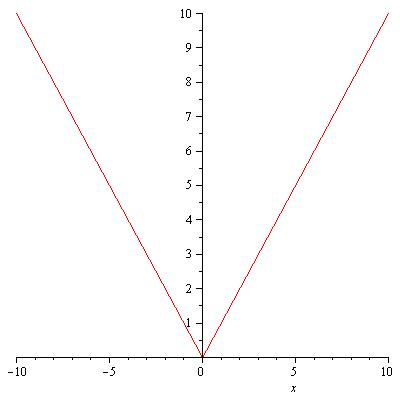
\includegraphics[width=0.50\textwidth]{abbildungen/abs(x).jpeg}
	\caption{$f(x) = |x|$}
	\label{fig:abs(x)}
\end{figure}
\end{bsp}
Erste Regel f�r die Ableitungsfunktion: 
\begin{equation*}
f(x)=x^n \rightarrow f'(x) = n \cdot x^{n-1}
\end{equation*}
Mit dieser Regel kann man Polynomfunktionen ableiten, denn es gilt zus�tzlich:
\begin{equation*}
(u(x)+v(x))' = u'(x) + v'(x)
\end{equation*}
\begin{bsp}
Die Ableitung der Funktion $f(x) = x^3 + 2x^2 + 4x -1$ lautet $f'(x) = 3x^2 + 4x + 4$.
\end{bsp}

\section {Eigenschaften einer Funktion}
\begin{itemize}
	\item Verhalten von $f$ f�r $ x \rightarrow \pm \infty $
	\item Nullstellen
	\item Monotonieverhalten
	\item	Extrema
	\item Wendepunkte
	\item Symmetrieverhalten
\begin{itemize}
	\item Nullpunktsymmetrie
	\item y-Achsensymmetrie
\end{itemize}
\end{itemize}

\section {Vollst�ndige Kurvendiskussion einer Ganz-Rationalen Funktion}
\begin{enumerate}
	\item Definitionsmenge\index{Definitionsmenge}, Differenzierbarkeit
	\item Ableitungen bilden
	\item Symmetrieverhalten \\
	Nullpunktsymmetrie: $ f(-x) = -f(x) $ \\
	y-Achsensymmetrie: $ f(-x) = f(x) $
	\item Verhalten f�r $ x \rightarrow \pm \infty $
	\item Nullstellen ($f(x) = 0$)
	\item Extrema (lokale) \\
	notwendige Bedingung: $ f'(x) = 0 $ \\
	hinreichende Bedingug: $f'(x) = 0 \land f''(x) \neq 0 $ \\
	a) $ f'(x_E) = 0 \land f''(x_E) < 0 \rightarrow $ in $x_E$ liegt ein HOP \\
	b) $ f'(x_E) = 0 \land f''(x_E) > 0 \rightarrow $ in $x_E$ liegt ein TIP
	\item Wendepunkte
	notwendige Bedingung: $f''(x) = 0$ \\
	hinreichende Bedingung: $f''(x) = 0 \land f'''(x) \neq 0$ \\
	a) $ f''(x_W) = 0 \land f'''(x_W) < 0 \rightarrow$  in $x_W$ liegt ein L-R Wendepunkt vor. \\
	b) $ f''(x_W) = 0 \land f'''(x_W) > 0 \rightarrow$  in $x_W$ liegt ein R-L Wendepunkt vor.
	\item Wertetabelle
	\item Graph
\end{enumerate}

\begin{bsp}[Diskussion der Funktion $f(x) = \frac{1}{3}x^3 + \frac{1}{2}x^2$]
Wir diskutieren hier als Beispiel die Funktion $f(x) = \frac{1}{3}x^3 + \frac{1}{2}x^2$ nach obigen Schema.
	\begin{enumerate}
		\item \textbf{Definitionsmenge} und \textbf{Diffbarkeit}: $D = \mathbb{R}$, da $f$ ein ganz-rationales Polynom, daher ist $f$ auch auf dem gesamten Definitionsbereich differenzierbar.
		\item \textbf{Ableitungen} bilden:
			\begin{align*}
				&f'(x) = x^2 + x\\
				&f''(x) = 2x+1\\ 
				&f'''(x) = 2
			\end{align*}
		\item \textbf{Symmetrie:} Das Polynom enth�lt sowohl gerade als auch ungerade Potenzen von x $\Rightarrow$ keine Aussagen �ber Symmetrie m�glich.
		\item \textbf{Nullstellen:}
			\begin{align*}
				&f(x) = \frac{1}{3}x^3 + \frac{1}{2}x^2 = x^2 \left(\frac{1}{3} x + \frac{1}{2}\right) \\
				\Rightarrow &f(x) = 0 \\
				\Leftrightarrow &x = 0 \vee \frac{1}{3} x + \frac{1}{2} = 0 \\
				\Leftrightarrow &x=0 \vee x = -\frac{3}{2}
			\end{align*}
			Die Nullstellen sind also $x_{N_1} = 0$ und $x_{N_2} = - \frac{3}{2}$.
		\item \textbf{Verhalten gegen $\pm \infty$:}\\
			\begin{align*}
				\lim_{x\to \infty} f(x) = + \infty\\
				\lim_{x\to - \infty} f(x) = - \infty
			\end{align*}
		\item \textbf{Extremstellen:}\\
			(1) notwendige Bedingung: $f'(x) = 0$\\
			(2) hinreichende Bedingung: $f''(x) \neq 0$\\
			zu (1):
			\begin{align*}
				f'(x) = 0 &\Leftrightarrow x^2 + x = 0\\
				&\Leftrightarrow x(x+1) = 0\\
				&\Leftrightarrow x=0 \vee x=-1
			\end{align*}
			zu (2):
			\begin{align*}
				f''(0) = 1 > 0 \Rightarrow \textrm{in $x=0$ liegt ein lokales Minimum}\\
				f''(-1) = -1 <0 \Rightarrow \textrm{in $x=-1$ liegt ein lokales Maximum}
			\end{align*}
		\item \textbf{Wendestellen:}\\
			(1) notwendige Bedingung: $f''(x) = 0$\\
			(2) hinreichende Bedingung: $f'''(x) \neq 0$\\
			zu (1):
			\begin{align*}
				f''(x) = 0 &\Leftrightarrow 2x + 1 = 0\\
				&\Leftrightarrow x = - \frac{1}{2}
			\end{align*}
			zu (2):
			\begin{align*}
				f'''\left(-\frac{1}{2}\right) = 2 >0 \Rightarrow \textrm{in $x = - \frac{1}{2}$ liegt ein Rechts-Links-Wendepunkt.}
			\end{align*}
		\item \textbf{Wertetabelle:}\\
			\begin{tabular}{c|c|c|c|c|c}
				$x$ & $-\frac{3}{2}$ & $0$ & $-1$ & $-\frac{1}{2}$ & $1$ \\
				\hline
				$f(x)$ & $0$ & $0$ & $\frac{1}{6}$&$\frac{1}{12}$&$\frac{5}{6}$\\
				\hline
				&Nst&Nst, Min& Max & WEP &
			\end{tabular}
		\item \textbf{Graph:}\\	
\begin{figure}[h]
	\centering
		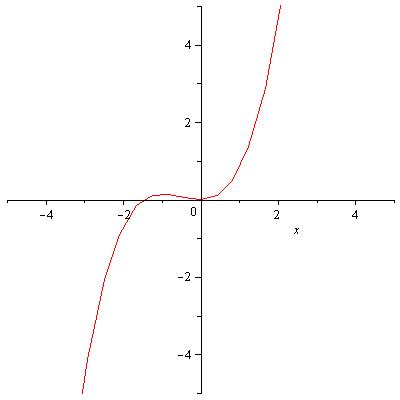
\includegraphics[width=0.50\textwidth]{abbildungen/funkt1.jpeg}
	\caption{$f(x) = \frac{1}{3}x^3 + \frac{1}{2}x^2$}
	\label{fig:funkt1}
\end{figure}
		
	\end{enumerate}
\end{bsp}

\section {Funktionenscharen}
$ f_a (x) = x^4 - ax^2$ --- $ a \in \mathbb{R} \land \mathbb{D}  \in \mathbb{R} $ \\
$a$ ist der Scharenparameter. Alle markanten Stellen  (Extrema, Wendepunkte, ...) werden in Abh�ngigkeit von $a$ berechnet.
\emph{Wichtig}: Gegebenenfalls sind Fallunterscheidungen notwendig!
\begin{definition}[Ortskurven]
\textbf{Ortskurven} sind Graphen, die durch jweils alle markanten Punkte eines Typs verlaufen. (Also zum Beispiel ein Graph durch alle WEP oder durch alle HOP usw.)
\end{definition}

\begin{bsp}[Diskussion einer Funktionenschar]
	Gegeben ist die Funktionenschar
	\begin{align*}
		f_a(x) = \frac{1}{4}x^4-ax^2 \quad a \in \mathbb{R}\setminus\{0\}
	\end{align*}
	\begin{enumerate}
		\item Wir bilden zun�chst die ersten drei \textbf{Ableitungen}:
			\begin{align*}
				f'_a(x) &= x^3 -2ax\\
				f''_a(x) &= 3x^2 -2a\\
				f'''_a(x) &=  6x
			\end{align*}
		\item \textbf{Symmetrie:} $f_a(x)$ ist achsensymmetrisch f�r alle $a$, denn es kommen nur gerade Potenzen von $x$ in der Funktionsgleichung vor.
		\item \textbf{Verhalten im Unendlichen:} Es ist
			\begin{align*}
				\lim_{x \to \infty} f_a(x) = \lim_{x \to \infty} \frac{1}{4}x^4 = \infty \\
				\lim_{x \to -\infty} f_a(x) = \lim_{x \to -\infty} \frac{1}{4}x^4 = \infty
			\end{align*}
		\item \textbf{Nullstellen:}
			\begin{align*}
				f_a(x) = 0 &\Leftrightarrow \frac{1}{4}x^4-ax^2 \\
				&\Leftrightarrow x^2 (\frac{1}{4} x^2 -a)\\
				&\Leftrightarrow x^2 = 0 \lor \frac{1}{4} x^2-a = 0 \\
				&\Leftrightarrow x = 0 \lor x = \pm 2\sqrt{a}
			\end{align*}
			Hier sehen wir nun, dass die Nullstellen abh�ngig von der Wahl des Parameters $a$ sind. Es ergibt sich:
			\begin{itemize}
				\item f�r $a<0$: $x=0$ ist die einzige Nullstelle, denn $2\sqrt{a}$ ist f�r $a<0$ nicht definiert.
				\item f�r $a>0$: Die Nullstellen sind $x=0$, $x=2\sqrt{a}$, $x=-2\sqrt{a}$
			\end{itemize}
		\item \textbf{Extrema:}
			\begin{align*}
				f'_a(x) = 0 &\Leftrightarrow x^3-2ax = 0\\
				&\Leftrightarrow x(x^2-2a) = 0\\
				&\Leftrightarrow x= 0 \lor x^2-2a = 0\\
				&\Leftrightarrow x= 0 \lor x^2 = 2a\\
				&\Leftrightarrow x= 0 \lor x = \pm \sqrt{2a}
			\end{align*}
			Wieder m�ssen wir die Extrema in Abh�ngigkeit von $a$ angeben:
			\begin{itemize}
				\item $a<0$: $x=0$ ist das einzige potentielle Extremum. Setze $x=0$ in $f''_a(x)$ ein und erhalte $f''_a(0) = -2a >0$ also ist $x=0$ in diesem Fall ein Tiefpunkt.
				\item $a>0$: Die Extrema sind $x=0$, $x=\sqrt{2a}$ und $x=-\sqrt{2a}$. Einsetzen in $f''_a(x)$ liefert, dass $x=\pm \sqrt{2a}$ Tiefpunkte sind und $x=0$ ein Hochpunkt.
			\end{itemize}
		\item \textbf{Wendestellen:}
			\begin{align*}
				f''_a(x) = 0 &\Leftrightarrow 3x^2 -2a = 0\\
				&\Leftrightarrow x^2 = \frac{2}{3}a\\
				&\Leftrightarrow x = \pm \sqrt{\frac{2}{3}a}
			\end{align*}
			\begin{itemize}
				\item $a<0$: Es gibt keine Wendepunkte.
				\item $a>0$: Die potentiellen Wendestellen sind $x=\pm \sqrt{\frac{2}{3}a}$. Durch Einsetzen in $f'''_a(x)$ erh�lt man, dass $\sqrt{\frac{2}{3}a}$ ein rechts-links Wendepunkt und $-\sqrt{-\frac{2}{3}a}$ ein links-rechts Wendepunkt ist.
			\end{itemize}
		\item \textbf{Ortskurve durch die Wendepunkte mit $x=\sqrt{\frac{2}{3}a}$ f�r $a>0$:}\\
			Die Wendepunkte haben die Koordinaten $W\left(\sqrt{\frac{2}{3}a}, - \frac{5}{9}a^2\right)$. Bringen wir nun $x$ und $y$ in funktionale Abh�ngigkeit:
			\begin{align*}
				x= \sqrt{\frac{2}{3}a} &\wedge y= - \frac{5}{9}a^2 \\
				a == \frac{3}{2} x^2 &\wedge y= - \frac{5}{9}a^2\\
				\Rightarrow y = - \frac{5}{4}x^4
			\end{align*}
			Die Ortskurve durch alle Wendepunkte mit $x=\sqrt{\frac{2}{3}a}$ lautet also $y = - \frac{5}{4}x^4$. Die Ortskurve durch die anderen Wendepunkte berechnet man analog.
		\item \textbf{Graph:}
\begin{figure}[h]
	\centering
		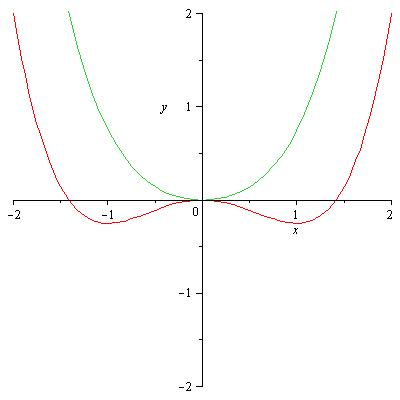
\includegraphics[width=0.70\textwidth]{abbildungen/funktschar1.jpeg}
	\caption{Die Graphen der Funktionenschar f�r $a=0.5$ (rot) und $a=-0.5$ (gr�n)}
	\label{fig:funktschar1}
\end{figure}		
	\end{enumerate}
\end{bsp}

\section{Bisher bekannte Ableitungsregeln}
\begin{enumerate}
	\item Konstantenregel \\
	$f(x) = c \cdot u(x)$, $u(x)$ differenzierbar und $ c \in \mathbb{R}$ \\
	$ \rightarrow $ f ist differenzierbar und 
	\begin{align}
	f'(x) = c \cdot u'(x)
	\end{align}
	\item Summenregel \\
	u, v differenzierbar \\
	$ f(x) = u(x) + v(x) $ differenzierbar und 
	\begin{align}
	f'(x) = u'(x) + v'(x)
	\end{align}
\end{enumerate}

\section {Weitere Ableitungsregeln}
\begin{satz}[Kettenregel]
Sei $f(x) = u(v(x)) $ und u, v differenzierbar, dann ist auch f differenzierbar und 
\begin{align} 
f'(x) = u'(v(x)) \cdot v'(x)
\end{align}
\end{satz}
\begin{bsp}
$f(x) = (x^2 + 3)^2$ also $u(x)=z^2$ und $ v(x) = x^2 + 3$
\begin{align*}
f(x)  &= x^4 + 6x^2 + 9 \\
f'(x) &= 4x^3 + 12x = 2(x^2 + 3) \\
\end{align*}
\end{bsp}
\begin{beweis}[Kettenregel]
$ x_0 \in \mathbb{D}_f $ beliebig, $ z = v(x)$ und $z_0 = v(x_0)$ ($z \neq z_0$ "`nahe"' $x_0$)
\begin{align*}
\lim_{x \rightarrow x_0} \left[ \frac{f(x) - f(x_0)}{x - x_0} \right] &= \lim_{x \rightarrow x_0} \left[ \frac{u(v(x)) - u(v(x_0))}{x-x_0} \cdot \frac{z-z_0}{z-z_0}\right] \\
&=\lim_{x \rightarrow x_0} \left[ \frac{u(z) - u(v(z_0))}{z-z_0}\right] \cdot  \lim_{x \rightarrow x_0} \left[ \frac{v(x) - v(x_0)}{x-x_0}\right] \\
&=\lim_{v(x) \rightarrow v(x_0)} \left[ \frac{u(z) - u(v(z_0))}{z-z_0}\right] \cdot v'(x_0)\\
&=u'(v(x_0)) \cdot v'(x_0)
\end{align*}
\end{beweis}

\begin{satz}[Produktregel]
Sei $ f(x) = u(x) \cdot v(x)$ und u, v sind differenzierbar. Dann gilt: f ist auch differenzierbar und 
\begin{align}
f'(x) = v(x) \cdot u'(x) + u(x) \cdot v'(x)
\end{align}
\end{satz}
\begin{bsp}
$f(x) = 2x^3 \cdot 4x$ also $u(x) = 2x^3 \Rightarrow u'(x) = 6x^2$ und $v(x) = 4x \Rightarrow v'(x) = 4$
\begin{align*}
f(x) &= 8x^4 \\
f'(x) &= 32x^3 \\
& = 24x^3 + 8x^3\\
& = 6x^2 \cdot 4x + 4 \cdot 2x^3 \\
\end{align*}
\end{bsp}
\begin{beweis}[Produktregel]
$ x_0 \in \mathbb{D}_f $ beliebig
\begin{align*}
\lim_{x \rightarrow x_0} \left[\frac{f(x) - f(x_0)}{x-x_0}\right] &= \lim_{x \rightarrow x_0} \left[\frac{u(x) v(x) - u(x_0)  v(x_0)}{x-x_0}\right]\\
&= \lim_{x \rightarrow x_0} \left[\frac{u(x)  v(x) - u(x_0)  v(x) + u(x_0)  v(x) - u(x_0)  v(x_0)}{x-x_0} \right] \\
&= \lim_{x \rightarrow x_0} \left[\frac{u(x)  v(x) - u(x_0)  v(x)}{x-x_0}\right]  \\
&\quad + \lim_{x \rightarrow x_0} \left[\frac{u(x_0)  v(x) - u(x_0)  v(x_0)}{x-x_0}\right]\\
&=v(x_0)  u'(x_0) + u(x_0)  v'(x_o)
\end{align*}
\end{beweis}

\begin{satz}[Quotientenregel]
Sei $f(x) = u(x) \cdot \frac{1}{v(x)}$ und u, v seien differenzierbar und $v(x) \neq 0$. Dann gilt: f ist auch differenzierbar und 
\begin{align}
f'(x) = \frac{v(x) \cdot u'(x) - u(x) \cdot v'(x)}{v^2(x)}
\end{align}
\end{satz}
\begin{beweis}[Quotientenregel]
\begin{align*}
f(x) &= u(x) \cdot \frac{1}{v(x)}\\
sei \quad \frac{1}{v(x)} &= w(x) \rightarrow w'(x) = - \frac{1}{v^2(x)} \cdot v'(x) \\
\\
f'(x) &= u'(x) \cdot w(x) + u(x) \cdot w'(x) \\
&= \frac{u'(x)}{v(x)} + u(x) \cdot \frac{-v'(x)}{v^2(x)}\\
&= \frac{v(x) \cdot u'(x) - u(x) \cdot v'(x)}{v^2(x)}
\end{align*}
\end{beweis}

\section{Extremalwertaufgaben mit Nebenbedingung}
\begin{enumerate}
	\item Skizze
	\item Extremale Gr��e als Formel erfassen (\emph{Extremalbedingung})
	\item Aufstellen einer \emph{Nebenbedingung}
	\item Reduktion der beiden Gleichungen auf eine Variable (\emph{Zielfunkrion})
	\item Berechnung des Extremums
	\item Hinreichende Bedingung pr�fen und / oder Randwerte betrachten
	\item R�ckbezug zum Sachproblem
\end{enumerate}

\section{Gebrochen rationale Funktionen}

\begin{definition}[Gebrochen-rationale Funktionen] Gebrochen-rationale Funktionen sind Quotienten aus zwei ganz-rationalen Funktionen.\\
$f(x) = \frac{u(x)}{v(x)}$, wobei $u$, $v$ differenzierbar und $n$ Grad von $u$, $m$ Grad von $v$.
\end{definition}

\begin{tabular}{|c|c|c|}
\hline
$n= m$:  \emph{unecht gebrochen} & $n<m$:  \emph{echt gebrochen} & $n>m$: \emph{unecht gebrochen}\\ \hline
$f(x) = \frac{2x^2 + 1}{3x^2 - 1}$ & $f(x) = \frac{x}{x^2+1}$ & $f(x) = \frac{x^2+3}{x-1}$\\ \hline
\end{tabular} \\
\\
F�r gebrochen-rationale Funktionen gilt: \\
$\mathbb{D} = \mathbb{R} \setminus \mathbf{N_v}$ \ \ ($ \mathbf{N_v}$: Nullstellenmenge von v) \\
$\mathbf{N_f} = \mathbf{N_u}$ \ \ (ein Bruch ist genau dann 0, wenn der Z�hler 0 ist.)

\subsection{Untersuchung einer Funktion in der N�he der Definitionsl�cken} \label{defluck}
Dieser Punkt ist bei der Diskussion einer gebrochen-rationalen Funktion gesondert zu betrachten.
\begin{definition}[Polstelle] Ist $x_0$ eine Nullstelle der Nennerfunktion und nach K�rzen \textbf{nicht} Nullstelle der Z�hlerfunktion, so hei�t $x_0$ \textbf{Polstelle} von $f$
\end{definition}
In der N�he von $x_0$ gilt dann: $f(x) \rightarrow \pm \infty $ \\
Wir unterscheiden:
\begin{enumerate}
	\item falls $x \rightarrow x_0 \land x<x_0$ \ \ \ $f(x) \rightarrow + \infty $ \\
	und $x \rightarrow x_0 \land x>x_0$ \ \ \ $f(x) \rightarrow + \infty $ \\
	dann hei�t $x_0$ \emph{Pol ohne Vorzeichenwechsel}.
	\item falls $x \rightarrow x_0 \land x<x_0$ \ \ \ $f(x) \rightarrow + \infty $ \\
	aber $x \rightarrow x_0 \land x>x_0$ \ \ \ $f(x) \rightarrow - \infty $ \\
	dann hei�t $x_0$ \emph{Pol mit Vorzeichenwechsel}.
\end{enumerate}

\subsection{Asymptotisches Verhalten}
\textbf{Wichtig:} Bei unecht gebrochen-rationalen Funktionen, deren Z�hlergrad h�her ist als der Nennergrad, ist zun�chst eine Polynomdivision durchzuf�hren, um ein ganz-rationales und ein echt gebrochen-rationales Polynom zu erhalten.
\begin{definition}[Asymptote] Eine Funktion $a(x)$ hei�t \emph{Asymptote} des Graphen f, genau dann wenn  $\lim_{x \to x_0} (f(x) - a(x)) = 0$
\end{definition}

\subsubsection{Erg�nzung: Regel von l'Hospital}
\begin{satz}[Regel von l'Hospital]
Sei $f(x) = u(x) / v(x)$ eine gebrochen rationale Funktion mit $v(x_0) = 0$. Sind $(u,v)$ differenzierbar in $x_0$, $u(x_0) = v(x_0) = 0$ und $v'(x_0) \neq 0$ dann ist
\begin{align}
\lim_{x \to x_0} \frac{u(x)}{v(x)} = \lim_{x \to x_0} \frac{u'(x)}{v'(x)}
\end{align}
\end{satz}

\subsection{Hebbare Definitionsl�cken}
\begin{definition}[Hebbare Definitionsl�cke] Ist $x_0$ eine Nullstelle des Nenners und auch Nullstelle des Z�hlers und l�sst sich der Linearfaktor $(x-x_0)$ vollst�ndig k�rzen, so hei�t $x_0$ \textbf{hebbare Definitionsl�cke}.
\end{definition}



\section{Ableitungen wichtiger Funktionen}



\begin{tabular}{c|c|c}
\textbf{Zeit} & \textbf{Wissende Personen} & \textbf{Wissende Personen} \\ \hline
$t=0$ & 1 & 3 \\ \hline
$t=1$ & 2 & 6 \\ \hline
$t=2$ & 4 & 12 \\ \hline
$t=3$ & 8 & 24 \\ \hline
Funktion: & $f(t) = 2^t$ & $f(t) = 2^t \cdot 3$ \\ \hline
\end{tabular}
\\
Allgemein: $f(x) = c \cdot a^x$ dabei ist $c$ der Startwert, $a$ der Wachstumsfaktor, $a 
 1$, $a \in \mathbb{R}^{+ \neq 1}$ ($0<a<1 \rightarrow$ Zerfall, $a>1 \rightarrow$ Wachstum) \\

\begin{satz} $f(x+1)=c \cdot a^{x+1} = c \cdot a \cdot a^x = a \cdot f(x)$ \end{satz}

\subsection{Ableitung von Exponentialfunktionen}
$f(x) = a^x$ \\
$a = e \rightarrow$ Eulerzahl \\
$f(x) = e^x \rightarrow$ Exponentialfunktion \\
\\
wobei: \\
$e= \lim_{n \rightarrow \infty} (1 + \frac {1}{n})^n$ mit $n \in \mathbb{N}$\\
f�r sehr gro�e $n$: $e\approx(1+\frac{1}{n})^n$ \\
$e\approx2.718$ \\
Ziel: Ableitung f�r $f(x) = a^x$\\
$x_0 \in \mathbb{D}$
\begin{align*}
f'(x) &= \lim_{x \rightarrow 0} \left[\frac{a^x - a^{x_0}}{x-x_0}\right]\\
&= \lim_{h \rightarrow 0} \left[\frac{a^{h+x_0}-a^{x_0}}{h}\right]\\
& = \lim_{h \rightarrow 0} \left[\frac{a^h \cdot a^{x_0} - a^{x_0}}{h}\right]\\
& = \lim_{h \rightarrow 0} \left[\frac{a^h - 1}{h}\right] \cdot a^{x_0}\\
\end{align*}
muss noch berechnet werden.\\

Spezialfall: $f(x) = e^x$
\begin{align*}
f'(x_0) &= e^{x_0} \cdot \lim_{h \rightarrow 0}\left[\frac{e^h - 1}{h}\right] \\
&= 1\\
& = \lim_{n \rightarrow \infty} \left[\displaystyle \frac{e^{\frac{1}{n}} - 1}{\frac{1}{n}}\right]
\end{align*}
\\
also bleibt zu zeigen, dass $\frac{e^{\frac{1}{n}} - 1}{\frac{1}{n}} = 1$ f�r sehr hohe $n$:
\begin{align*}
&\Leftrightarrow e^{\frac{1}{n}} -1 = \frac {1}{n} \\
&\Leftrightarrow e^{\frac{1}{n}} = \frac {1}{n} + 1 \\
&\Rightarrow e = (\frac{1}{n} + 1)^n \\
&\Rightarrow f'(x) = f(x)
\end{align*}

\subsection{Nat�rliche Logarithmusfunktion}
$e^x \rightarrow \overline{f}(x) = \ln(x)$: Nat�rliche Logarithmusfunktion. \\
$y=e^x \rightarrow x = \ln(y)$ \\
$a = e^{\ln(a)}$ allgemeing�ltig \\

Daraus l�sst sich eine allgemeing�ltige Ableitung von Exponentialfunktionen entwickeln:
\begin{align*}
f(x) &= a^x \\
&= (e^{(\ln(a))^x}\\ 
&= e^{\ln(a) x} \\
\Rightarrow f'(x) &= e^{\ln(a) x} \cdot \ln(a)\\
&= \ln(a) \cdot a^x
\end{align*}
\\
Zusammenfassend:\\
$(a^x)' = a^x \cdot \ln(a)$ \\
$(e^x)' = e^x$ \\
$f(x) = a^x \Leftrightarrow f(x) = e^{\ln(a)x}$ \\
Es gen�gt also, die e-Funktion genau zu kennen, und zu diskutieren.

\subsubsection{Ableitung der Logarithmusfunktion}

$f(x) = \ln(x)$ \\
\begin{align*}
x&=e^{\ln(x)} \\
1&=e^{\ln(x)} \cdot \ln'(x)\\
ln'(x) &= \frac{1}{e^{\ln(x)}} \\
& = \frac{1}{x}
\end{align*}

\subsection{Trigonometrische Funktionen}

\emph{Additionstheoreme:}\\
1. $\sin(\alpha) - \sin(\beta) = 2\cos(\frac{\alpha + \beta}{2}) \cdot \sin(\frac{\alpha - \beta}{2})$ \\
2. $\cos(\alpha) - \cos(\beta) = 2\sin(\frac{\alpha + \beta}{2}) \cdot \cos(\frac{\alpha - \beta}{2})$\\
\\
Vermutung: $sin'(x) = cos(x)$ \\
\begin{beweis}
$x_0 \in \mathbb{D}_{sin} = \mathbb{R}$ \\
\begin{align*}
\lim_{x \rightarrow x_0} \left[\frac{f(x)-f(x_0)}{x-x_0}\right] = \lim_{x \rightarrow x_0} \left[\frac{\sin(x) - \sin(x_0)}{x-x_0}\right]
\end{align*}

Sei $x:=x_0 + h \Rightarrow x-x_0 = h$, statt $x\rightarrow x_0$ nun $h \rightarrow 0$.

\begin{align*}
&=\lim_{h \rightarrow 0}\left[\frac{\sin(x_0 + h) - \sin (x_0)}{h}\right]\\
&=\lim_{h \rightarrow 0}\left[\displaystyle \frac{2\cos(\frac{x_0 +h + x_0}{2}) \cdot \sin(\frac{x_0 + h + x_0}{2})}{h}\right]\\
&=\lim_{h \rightarrow 0}\left[\displaystyle \frac{\cos(x_0 + \frac{h}{2}) \cdot \sin(\frac{h}{2})}{\frac{h}{2}}\right] = \cos(x_0) \\
\end{align*}

Es folgen analog:\\
$\cos'(x) = -\sin(x)$\\
$\tan'(x) = \frac{1}{cos^2(x)}$
\end{beweis}


%\chapter{Differentialrechnung mit gebrochen-rationalen Funktionen} \label{gebr}
%\input{differentialrGRFkt.tex}

\chapter{Integralrechnung}
\section{Die Streifenmethode} \label{streifen}
\begin{figure}[h]
	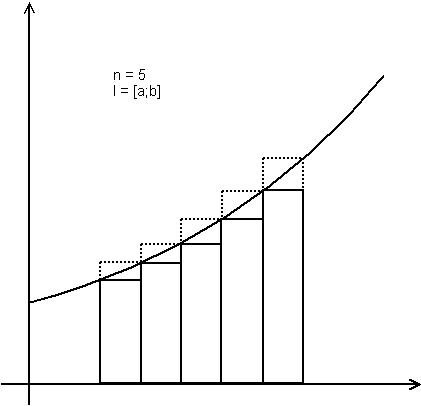
\includegraphics[width=0.75\textwidth]{abbildungen/int1.jpg}
	\caption{Streifenmethode}
	\label{fig:int1}
\end{figure}
\begin{itemize}
	\item Einbeschriebene Rechteckfl�chen $\rightarrow$ Untersumme $U_5$
	\item Umbeschriebene Rechteckfl�chen $\rightarrow$ Obersumme $O_5$
	\item Verfeinerung der Intervalleinteilung auf n gleiche Intervallabschnitte $U_n$, $O_n$
	\item $n \rightarrow \infty$
	\item ${\lim}_{n \rightarrow \infty} [U_n] = {\lim}_{n \rightarrow \infty} [O_n] = A^b _a$
\end{itemize} 
\begin{bsp}
$ f(x) = x$ \\
\begin{figure}[h]
	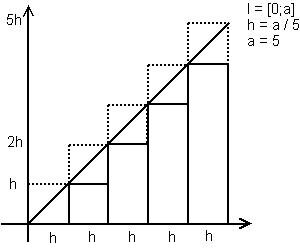
\includegraphics[width=1.00\textwidth]{abbildungen/int2.jpg}
	\caption{$f(x) = x$}
	\label{fig:int2}
\end{figure}
\end{bsp}

\textbf{Einschub \ref{streifen}.1:} Das Summenzeichen
\begin{align*}
1+2+3+4 &= \sum \limits_{\nu = 1}^4 \nu = 10 \\
1+2+3+4+...+n &= \sum \limits_{\nu = 1}^n \nu \\
\end{align*}

\begin{align*}
&U_5 = 1hh +2hh+3hh+4hh = h^2 \cdot (1+2+3+4) = \frac{a^2}{5^2} \cdot \sum \limits_{\nu = 1}^4 \nu \\
&O_5 = 1hh +2hh+3hh+4hh+5hh = h^2 \cdot (1+2+3+4+5) = \frac{a^2}{5^2} \cdot \sum \limits_{\nu = 1}^5 \nu \\
&U_n = \frac{a^2}{n^2} \cdot \sum \limits_{\nu = 1}^{n-1} \nu \\
&O_n = \frac{a^2}{n^2} \cdot \sum \limits_{\nu = 1}^{n} \nu \\
\end{align*}


\textbf{Einschub \ref{streifen}.2:} \\
$\sum \limits_{\nu = 1}^{n} \nu = \frac{n(n+1)}{2}$\\


\begin{align*}
U_n &= \frac{a^2}{n^2} \cdot \frac{(n-1)n}{2}\\
&= \frac{a^2}{2} \cdot \frac{n^2-n}{n^2}\\
O_n &= \frac{a^2}{n^2} \cdot \frac{n(n+1)}{2}\\
&= \frac{a^2}{2} \cdot \frac{n^2+n}{n^2}\\
\lim_{n \to \infty} U_n &= \lim_{n \to \infty} \left[\frac{a^2}{2} \cdot \frac{n^2-n}{n^2}\right]\\
&= \lim_{n \to \infty}\left[\frac{a^2}{2} \cdot (1-\frac{1}{n})\right] = \frac{a^2}{2}\\
\lim_{n \to \infty} O_n &= \lim_{n \to \infty} \left[\frac{a^2}{2} \cdot \frac{n^2+n}{n^2}\right]\\
&= \lim_{n \to \infty}\left[\frac{a^2}{2} \cdot (1+\frac{1}{n})\right] = \frac{a^2}{2}
\end{align*}
\\
F�r $ f(x) = x$ gilt also $A^a _0 = \frac{a^2}{2}$ also $A_a ^b = A_0^b - A_0^a = \frac{b^2}{2} - \frac{a^2}{2}$ \\
entsprechend gilt f�r $f(x) = x^2$: $A_0^a = \frac{a^3}{3}$ und so weiter... 

\section{Stammfunktionen}
$F(x) = \frac{x^2}{2} \rightarrow F'(x) = f(x)$\\
$F(x)$ ist die Stammfunktion von $f(x)$ \\
\begin{definition}[Stammfunktion] Eine differenzierbare Funktion $F$ hei�t \textbf{Stammfunktion} zu einer Funktion $f$, genau dann wenn gilt: $F'(x)  =f(x)$
\end{definition}
\begin{tabular}{l|l}
\hline
\textbf{Funktion} & \textbf{Stammfunktion} \\
\hline
$f(x) = x^2$ & $F(x) = \frac{1}{3} x^3$ oder $G_{17} (x)= \frac{1}{3} x^3 + 17$ oder $G_c (x) = F(x) + c$ \\ \hline
\end{tabular}
\\
\\
$A_a ^b= \frac{1}{3} x^3 +5 ]^b _a = \frac{1}{3} b^3 + 5 - (\frac{1}{3} a^3 + 5)$ \\
\\
Stammfunktion $F$ $\rightarrow$ unendliche viele \\
Grundfunktion $f$ \\
Ableitungsfunktion $f'$ $\rightarrow$ eindeutig
\subsection {Eigenschaften von Stammfunktionen}
(Ziel: Bildung von Stammfunktionen folgender Funktionen) \\
(Voraussetzung: $U$ Stammfunktion von $u$, $V$ Stammfunktion von $v$) 
\\
\begin{tabular}{l|l}
\textbf{Funktion} & \textbf{Stammfunktion} \\ \hline
$f(x) = x^n \land n \in \mathbb{R}^{\neq-1}$ & $F(x) = \frac{1}{n+1} \cdot x^{n+1}$ \\ \hline
$f(x) = c \cdot u(x)$ & $F(x) = c \cdot U(x)$ \\ \hline
$f(x) = u(x) + v(x)$ & $F(x) = U(x) + V(x)$ \\ \hline
$f(x) = x^{-1}$ & noch nicht mglich \\ \hline
$f(x) = u(x) \cdot v(x)$ & noch nicht m�glich \\ \hline
$f(x) = u(rx + b)$ (lineare Verkettung) & $F(x) = \frac{1}{r} U (rx+b)$ \\ \hline
\end{tabular}

\section{Bestimmte Integrale}
Beliebige Funktion $f$ (stetig, d.h. "`ohne L�cke und Sprung"') \\
Unterteilt in $n$ gleiche Teilintervalle $[a,b]$ der Breite $\Delta x$ \\
\begin{align*}
&U_n = \sum \limits_{\nu = 0}^{n-a} f(a+ \nu \Delta x) \Delta x \\
&O_n = \sum \limits_{\nu = 1}^{n} f(a+ \nu \Delta x) \Delta x  \\
&\lim_{n \to \infty} U_n = \int \limits_{a}^{b} f(x)dx \\
&\lim_{n \to \infty} O_n = \int \limits_{a}^{b} f(x)dx\\
\end{align*}

\subsection{Eigenschaften des bestimmten Integrals}
\begin{enumerate}
	\item $\int \limits_{a}^{a} f(x) dx = 0$
	\item Faktorregel: $k \cdot \int \limits_{a}^{b} f(x) dx = \int \limits_{a}^{b} k \cdot f(x) dx$
	\item Summenregel: $\int \limits_{a}^{b} f(x) + g(x) dx = \int \limits_{a}^{b} f(x) dx + \int \limits_{a}^{b} g(x) dx$
	\item Grenzen vertauschen: $\int \limits_{a}^{b} f(x) dx = -\int \limits_{b}^{a} f(x) dx$
	\item Intervalladditivit�t: $\int \limits_{a}^{b} f(x) dx = \int \limits_{a}^{c} f(x) dx + \int \limits_{c}^{b} f(x) dx$ wenn $a<c<b$
	\item Monotonie des Integrals: \\ $f(x) \leq g(x)$ auf $I = [a,b] \Rightarrow \int \limits_{a}^{b} f(x) dx \leq \int \limits_{a}^{b} g(x) dx$
	\item $\int \limits_{a}^{b} f(x) dx = \int \limits_{a}^{b} f(t) dt$
	\item falls $f(-x) = -f(x) \land x \in I=[a,b]$ dann $\int \limits_{-a}^{a} f(x) dx = 0$
\end{enumerate}

\section {Fl�che zwischen Graph und x-Achse}
Wenn der Graph auf $I=[a,b]$ \emph{keine} Nullstelle besitzt, dann errechnet man die Fl�che wie folgt: \\
$A =  \left| \int \limits_{a}^{b} f(x) dx \right|$ \\
Besitzt der Graph auf $I=[a,b]$ Nullstellen, so muss der Intervall in Teilintervalle unterteilt werden. Sei zum Beispiel $c$ die (einzige) Nullstelle von $f(x)$. Dann ist die Fl�che $A= \left| \int \limits_{a}^{c} f(x) dx \right| + \left| \int \limits_{c}^{b} f(x) dx \right|$

\section{Fl�che zwischen zwei Graphen}
\subsection{... die sich auf [a,b] nicht schneiden}
$A= \left| \int \limits_{a}^{b} f(x) - g(x) dx \right|$
\subsection{... die sich auf [a,b] schneiden}
\begin{enumerate}
	\item Schnittpunkte berechnen
	\item Teilfl�chen berechnen
	\item Teilfl�chen aufaddieren
\end{enumerate}

\section{Menge aller Integralfunktionen}
$I_a (x) = \int \limits_{a}^{x} f(x) dx = F(x)]^x_a=F(x) - F(a)$

\section{Hauptsatz der Integral und Differentialrechnung}
\begin{satz}[Hauptsatz der Integral- und Differentialrechnung]
Sei $f$ eine auf $I=[a,b]$ stetige Funktion. Dann gilt f�r die Funktion $I_a$ mit $I_a = \int \limits_{a}^{x} f(t) dt$:
\begin{align*}
I'_a (x) &= f(x) \\
\int \limits_{a}^{b} f(x) dx &= F(b) - F(a) \in \mathbb{R}
\end{align*}
\end{satz}

\section{Einschub: Vollst�ndige Induktion (LK)} \label{vollind}
\emph{Axiom von Peano:}\\
$M$ Menge. \\
\begin{align*}
1 \in M \land (n \in M \Rightarrow n+1 \in M) \Rightarrow M = \mathbb{N}
\end{align*}
\\
\begin{bsp}
Summe aller ungeraden Zahlen: $ 1+3+5+...+(2n-1) = n^2$
\begin{beweis}

\begin{enumerate}
	\item Verankerung: \\ 
	$A_{(1)}$ ist wahr, denn $1 = 1^2$
	\item Schluss von $n$ auf $n+1$: \\
	$A_{(n+1)}$ ist wahr unter Verwendung der Wahrheit von $A_(n)$ \\
	$A_{(n+1)}$: \\
	$1+3+5+...+(2(n+1)-1) = (n+1)^2$ \\
	$\Leftrightarrow 1+3+5+...+(2n-1) + (2(n+1)-1) = (n+1)^2$ \\
	$\Leftrightarrow n^2 + (2(n+1)-1)=(n+1)^2$\\
	$\Leftrightarrow n^2 + 2n + 1 = (n+1)^2$ \\
	$\Leftrightarrow (n+1)^2 = (n+1)^2$
	\item Nach Peano Axiom gilt damit: $A_{(n)} \forall n \in \mathbb{N}$
\end{enumerate}
\end{beweis}
\end{bsp}

\section{Rotationsk�rper (LK)}
... sind K�rper, die durch die Rotation einer Fl�che um eine Achse entstehen. \\
Ziel: Berechnung des Volumens mit Hilfe der Integralrechnung. \\
\\
Sei $f$ auf $I=[a,b]$ stetig. \\
Gesamtvolumen $\rightarrow$ unendlich viele Zylinder.
\begin{align*}
V&= \lim_{n \to \infty}  \sum \limits_{}^{n-1} \pi f^2(x) dx\\
&= \pi \int \limits_{a}^{b} f^2(x) dx
\end{align*}
= Volumen eines Rotationsk�rper, der durch $f$ erzeugt wird. \\
Wird z.B. benutzt, um das Volumen einer Kugel herzuleiten! \\
F�r einen Rotationsk�rper, der von zwei Funktionen vorgegeben wird, gilt:
\begin{align*}
V&= \pi \int \limits^{b}_{a} f^2(x)dx - \pi \int \limits^{b}_{a} g^2(x)dx \\
&= \pi \int \limits^{b}_{a} f^2(x) - g^2(x)dx
\end{align*}


\section{Weitere Integrationsregeln (LK)}


\subsection{Partielle Integration}
Dient zum Integrieren von Produkten von Funktionen. \\
Produktregel: $(u(x) \cdot v(x))' = v'(x) u(x) + u'(x) v(x)$ $u, v$ differenzierbar und stetig; $u', v'$ stetig \\
\begin{align*}
u(x) v'(x) &= (u(x) v(x))' - u'(x) v(x) \\
\Leftrightarrow \int \limits_{a}^{b} {u(x) v'(x)dx} &= \int \limits_{a}^{b} {(u(x) v(x))' dx} - \int \limits_{a}^{b} {u'(x)v(x)dx}
\end{align*}
Dies f�hrt zu folgender Regel zum Integrieren von Produkten von Funktionen:
\begin{align}
\int \limits_{a}^{b} {u(x) v'(x)dx} = u(x) \cdot v(x) ]_a ^b - \int \limits_{a}^{b} {u'(x)v(x)dx}
\end{align}


\subsection{Integration durch Substitution}
(Basiert auf der Kettenregel der Differentialrechnung) \\
Kettenregel: \\
$u \circ v(x) = u(v(x))$; u, v diffbar \\
$(u \circ v(x)') = (u(v(x)))' = u'(v(x) \cdot v'(x))$ \\

Sei $U$ Stammfunktion von $u$: $U'(x) = u(x)$
\begin{align*}
(U(x))' &= U'(v(x)) \cdot v'(x) = u(v(x) \cdot v'(x)\\
\Rightarrow \int \limits_{a}^{b} {u(v(x)) \cdot v'(x)}dx &= \int \limits_{a}^{b} {U'(v(x))}dx = U(v(x))]_a ^b = U(v(b)-U(v(a))
\end{align*}

Substitution: $ = U(z)]_{v(a)}^{v(b)}$ \\
Daraus ergibt sich folgende Regel:
\begin{align}
\int \limits_{a}^{b} {u(v(x)) \cdot v'(x)}dx = U(z)]_{v(a)}^{v(b)}
\end{align}

\part{Lineare Algebra}

\chapter{Lineare Gleichungssysteme (LGS)}
\[ a_1 x_1 + a_2 x_2 + a_3 x_3 + ... + a_n x_n = b \] hei�t \emph{lineare Gleichung} \\
\begin{tabular} {ll}
$x_i$ & Variablen \\
$a_i$ & Koeffizienten \\
$b$ & absolut gleich
\end{tabular}\\
$x_i$ sind stets linear (1. Potenz)

\section{Allgemeines Gleichungssystem}
\[ a_{11} x_1 + a_{12} x_2 + \ldots + a_{1n} x_n = b_1 \]
\[ a_{21} x_1 + a_{22} x_2 + \ldots + a_{2n} x_n = b_2 \]
\[ \vdots \]
\[ a_{m1} x_1 + a_{m2} x_2 + \ldots + a_{mn} x_n = b_n \]
$n$ Unbekannte \\
$m$ Gleichungen \\
$a_{ij}$ hei�en \emph{Koeffizienten}

\section{Koeffizientenmatrix}
\[ \left( \begin{array}{ccccc|c}
a_{11} & a_{22} & a_{33} & \ldots & a_{1n} & b_1 \\
a_{21} & a_{22} & a_{23} & \ldots & a_{2n} & b_2 \\
			 &				&				 & \vdots & 			 & 	\vdots \\
a_{m1} & a_{m2} & a_{m3} & \ldots & a_{mn} & b_n
\end{array}\right) \]
wobei $a_{1j}$ die Koeffizienten der Unbekannten in der ersten Gleichung sind, $a_{2j}$ die Koeffizienten in der zweiten Gleichung usw.

\section{Gau�-Verfahren}
Das Gau�-Verfahren dient zur �berf�hrung einer Matrix in Zeilenstufenform, sodass das zugeh�rige LGS einfach zu l�sen \begin{bsp}
\begin{align*}
\left( \begin{array}{ccc|c}
1 & 2 & 3 & 7 \\
0 & 4 & 0 & 6 \\
0 & -4 & -3 & -7 \\
\end{array}\right) \\
\left( \begin{array}{ccc|c}
1 & 2 & 3 & 7 \\
0 & 4 & 0 & 6 \\
0 & 0 & -3 & -1 \\
\end{array}\right) \\
\end{align*}
Diese Matrix ist in Zeilenstufenform, da sich unterhalb der Hauptdiagonalen (1, 4, -3) nur Eintr�ge = 0 befinden. Das Gleichungssystem ist nun einfach zu l�sen. \\
\end{bsp}

Erlaubte Umformungen im Gau�-Verfahren: \\
\begin{itemize}
	\item Zeilen komplett vertauschen. ($\stackrel{I \leftrightarrow III}{\longrightarrow}$)
	\item Multiplikation einer Gleichung mit einer Zahl verschieden von Null. ($\stackrel{I \cdot \lambda}{\longrightarrow}$)
	\item Addition von zwei Gleichungen. ($\stackrel{I + III}{\longrightarrow}$)
\end{itemize}

\subsection{Verschiedene F�lle}
An drei Beispielen:

\begin{bsp}
$\left( \begin{array}{cc|c}
2 & -1 & 1 \\
0 & 4 & 1
\end{array} \right)$
eindeutig l�sbar
\end{bsp}

\begin{bsp}
$\left( \begin{array}{ccc|c}
1 & -2 & -4 & 2 \\
0 & 3 & 2 & 0 \\
0 & 0 & 0 & -1
\end{array} \right)$
nicht l�sbar ($-1 \neq 0$)
\end{bsp}

\begin{bsp}
$\left( \begin{array}{ccc|c}
2 & -1 & 1 & 2 \\
0 & 2 & -6 & 0 \\
0 & 0 & 0 & 0
\end{array} \right)$\\
unendlich viele L�sungen (zwei linear abh�ngige Zeilen)\\
\begin{align*}
\mathbb{L} = \{ (1 - r | 3r | r)|r \in \mathbb{R} \}
\end{align*}
wobei $r$ \emph{L�sungsparameter} genannt wird.
\end{bsp}

\section{LGS mit Parameter (Schar von LGS)}
\[
\begin{array}{l}
	x_1 + x_2 - 2x_3 = 0 \\
	2x_1 - 2x_2 + 3x_3 = 1 + 2t \\
	x_1 - x_2 - x_3 = t
\end{array}
\]
$t$ hei�t \emph{Scharparameter} $\rightarrow$ unendlich viele lineare Gleichungssysteme\\
\textbf{Wichtig:} Beim L�sen eines solchen Systems m�ssen unter Umst�nden Fallunterscheidungen gemacht werden! (Nicht durch Null teilen!)

\section{Erweitertes Gau�-Verfahren}
Beim erweiterten Gau�-Verfahren versuchen wir, die Matrix nicht nur in Zeilenstufenform zu bringen, sondern sie zur \textit{Einheitsmatrix} umzuformen. \\
Wir m�ssen die Matrix also so umformen, dass alle Eintr�ge Null sind, au�er diejenigen auf der Diagonalen und diese sind gleich 1.\\

Beispiel f�r ein 3x3 System nach dem erweiterten Gau�-Verfahren:
\begin{bsp}
$\left( \begin{array}{ccc|c}
1 & 0 & 0 & b_1 \\
0 & 1 & 0 & b_2 \\
0 & 0 & 1 & b_3
\end{array} \right)$\\

Die L�sungen lassen sich nun ganz einfach ablesen:\\
$x_1 = b_1$ \\
$x_2 = b_2$ \\
$x_3 = b_3$
\end{bsp}

\chapter{Vektoriell-analytische-Geometrie}
$\rightarrow$ geometrische Beziehungen und Sachverhalte arithmetisch erfasst und untersucht.

\section{Einf�hrung des Vektorbegriffs}
Ein Vektor im geometrischen Sinne ist eine Art "`Abbildung"' von einem Punkt zum andern.\\
Name eines Vektors (Pfeils): 
\[ \vec{PP'} = \vec{a} \]
Pfeil $\Rightarrow$ Pfeilklasse = Vektor\\

Vektoren unterscheiden sich durch:
\begin{itemize}
	\item unterschiedliche Richtung
	\item unterschiedliche Orientierung
	\item unterschiedliche L�nge
\end{itemize}

Weitere Definitionen:
\begin{itemize}
	\item L�nge eines Vektors $ |\vec{a}| = |-\vec{a}|$
	\item $\vec{PP} = \vec{0}$ Nullvektor mit $\vec{a} + \vec{0} = \vec{a}$
	\item $\vec{a} = \vec{b} \Leftrightarrow $ $\vec{a}$ und $\vec{b}$ haben dieselbe L�nge, dieselbe Orientierung und dieselbe Richtung.
\end{itemize}

\section{Vektoraddition}
Vektoren werden addiert, indem man den Schaft des zweiten Vektors an die Spitze des ersten Vektors legt. Der \emph{resultierende} Vektor hat dann den Schaft des ersten Vektors und die Spitze in der Spitze des zweiten Vektors.
\subsection{L�nge von Summenvektoren}
\begin{tabular}{lcl}
$\vec{a} \uparrow \uparrow \vec{b}$ & : & $|\vec{a} + \vec{b}| = |\vec{a}| + |\vec{b}|$ \\
$\vec{a} \uparrow \downarrow \vec{b}$ & : & $|\vec{a} + \vec{b}| = ||\vec{a}| - |\vec{b}|| \leq  |\vec{a}| + |\vec{b}|$ \\
$\vec{a} / / \vec{b}$ & : & $|\vec{a} + \vec{b}| \leq |\vec{a}| + |\vec{b}|$ (\emph{Dreiecksungleichung})
\end{tabular}

\section{Skalarmultiplikation}
\label{Skalarmultiplikation}
\begin{definition}[Skalar] Unter einem \textbf{Skalar} versteht man i.d.R. eine reelle Zahl. \end{definition}
\subsection{Gesetze zur Skalarmultiplikation}
F�r alle $\lambda, \mu \in \mathbb{R}$ und alle $\vec{a}, \vec{b} \in V$ (V = Vektorraum. siehe unten.) gilt:\\
\begin{itemize}
	\item $\lambda \cdot (\mu \cdot \vec{a}) = (\lambda \mu) \cdot \vec{a}$
	\item $(\mu + \lambda) \cdot \vec{a} = \mu \vec{a} + \lambda \vec{a}$
	\item $ \lambda (\vec{a} + \vec{b}) = \lambda \vec{a} + \vec{b}$
	\item $ \lambda \vec{0} = \vec{0}$
	\item $ \lambda \vec{a} = 0 \Leftrightarrow \lambda = 0 \lor \vec{a} = 0$\\
\end{itemize}

\section{Vekorr�ume (LK)}
\label{Vraum}\begin{definition}[Vektorraum] Eine nicht leere Menge $V$ nennt man einen \textbf{Vektorraum} und ihre Elemente \textbf{Vektoren}, wenn
\begin{enumerate}
	\item es eine "`Addition"' gibt, die Elementen $\vec{a}, \vec{b} \in V$ jeweils genau ein Element $\vec{a} + \vec{b} \in V$ zuordnet, und hierbei gilt:
	\begin{enumerate}
		\item Es gibt ein "`Nullelement"' $\vec{0} \in V$ mit $\vec{a} + \vec{0} = \vec{a}$ f�r alle $\vec{a} \in V$
		\item Zu jedem $\vec{a} \in V$ gibt es ein "`Gegenelement"' $-\vec{a} \in V$ mit $\vec{a} + (-\vec{a}) = \vec{0}$
		\item F�r alle $\vec{a}, \vec{b}, \vec{c} \in V$ gilt $\vec{a} + (\vec{b} + \vec{c}) = (\vec{a} + \vec{b}) + \vec{c}$ (Assoziativgesetz)
		\item F�r alle $\vec{a}, \vec{b} \in V$ gilt: $\vec{a} + \vec{b} = \vec{b} + \vec{a}$ (Kommutativgesetz)
	\end{enumerate}
	\item es eine "`Multiplikation"' gibt, die jeweils einer reellen Zahl $\lambda$ und einem Element $\vec{a} \in V$ genau ein Element $\lambda \cdot \vec{a} \in V$ zuordnet und hierbei gilt:
	\begin{enumerate}
	\item F�r alle $\lambda \in \mathbb{R}$, $\vec{a}, \vec{b} \in V$ gilt: $\lambda \cdot (\vec{a} + \vec{b}) = \lambda \vec{a} + \lambda \vec{b}$ und f�r alle $\lambda, \mu \in \mathbb{R}$, $\vec{a} \in V$ gilt: $(\lambda + \mu) \cdot \vec{a} = \lambda \vec{a} + \mu \vec{a}$. (Distributivgesetze)
	\item F�r alle $\lambda, \mu \in \mathbb(R)$, $\vec{a} \in V$ gilt: $\lambda \cdot (\mu \cdot \vec{a}) = (\lambda \cdot \mu) \cdot \vec{a}$. (Assoziativgesetz)
	\item F�r alle $\vec{a} \in V$ gilt: $ 1 \cdot \vec{a} = \vec{a}$.
\end{enumerate}
\end{enumerate}
\end{definition}

\section{Vektorketten}
\begin{definition}[Vektorkette] Die Summe aus endlich vielen Vektoren hei�t \textbf{Vektorkette}.\end{definition}

Offene Vektorkette: $ \vec{a} + \vec{c} + \vec{d} = \vec{x}$ \\
Geschlossene Vektorkette: $\vec{a} + \vec{c} + \vec{d} = \vec{0}$\\
Jede offene Vektorkette l�sst sich schlie�en, indem man den Gegenvektor des resultierenden Vektors addiert: $\vec{a} + \vec{c} + \vec{d} + (-\vec{x}) = \vec{0}$

\section{Linearkombinationen}
\begin{definition}[Linearkombination]
\[ \lambda_1 \vec{a_1} + \lambda_2 \vec{a_2} + \ldots + \lambda_n \vec{a_n} = \vec{x}\]
mit $\lambda_1, \ldots, \lambda_n \in \mathbb{R}$ und $\vec{a_1}, \ldots, \vec{a_n} \in \mathbb{R}$ hei�t Linearkombination aus den Vektoren $\vec{a_1}, \ldots, \vec{a_n}$\\
Oder anders: 
\[ \vec{x} = \sum \limits_{i=1} ^{n} {\lambda_i a_i}\]
\end{definition}

\section{Vektorr�ume (Beispiele) (LK)}
Ebene $\mathbb{R}^2$ \\
Raum $\mathbb{R}^3$ \\

\textbf{Ebene}: \\
$P (P_1 | P_2)$ \\
Ortsvektor zu P: $ \vec{0p} = \vec{p} = \left( \begin{array}{cc} p_1 \\ p_2 \end{array} \right)$ \\
\[ \mathbb{R}^2 = \{ \left( \begin{array}{c} x_1 \\ x_2 \end{array} \right) | x_1 , x_2 \in \mathbb{R} \} \] 
ist ein Vektorraum.\\

\textbf{Raum}: \\
$P (P_1 | P_2 | P_3)$ \\
$x_1$-$x_2$ - Ebene\\
$x_2$-$x_3$-Ebene\\
$x_1$-$x_3$-Ebene\\
Ortsvektor zu P: $ \vec{0p} = \vec{p} = \left( \begin{array}{c} p_1 \\ p_2 \\ p_3 \end{array} \right)$ \\
\[ \mathbb{R}^3 = \{ \left( \begin{array}{c} x_1 \\ x_2 \\x_3 \end{array} \right) | x_1 , x_2 , x_3 \in \mathbb{R} \} \] 
ist ein Vektorraum.\\

Allgemein (\textbf{n-Tupel}): \\
\[ \mathbb{R}^n = \{ \left( \begin{array}{c} x_1 \\ x_2 \\ \vdots \\ x_n \end{array} \right) | x_1 , x_2 , \ldots , x_n \in \mathbb{R} \} \] 
ist ein Vektorraum. (wobei $n \in \mathbb{N}$)\\

\begin{definition}[Addition im $\mathbb{R}^n$]
Seien $\vec{a} = \left( \begin{array}{c} a_1 \\ a_2 \\ \vdots \\ a_n \end{array} \right), \vec{b} = \left( \begin{array}{c} b_1 \\ b_2 \\ \vdots \\ b_n \end{array} \right) \in \mathbb{R}^n$. Dann gilt: $\vec{a} + \vec{b} = \left( \begin{array}{c} a_1 + b_1 \\ a_2 + b_2 \\ \vdots \\ a_n + b_n \end{array} \right)$
\end{definition}

\begin{definition}[Skalarmultiplikation im $\mathbb{R}^n$]
Seien $ \lambda \in \mathbb{R}, \vec{v} \in \mathbb{R}^n$. Dann gilt: $\lambda \vec{v} = \lambda \left( \begin {array}{c} v_1 \\ v_2 \\ \vdots \\ v_n \end{array} \right) = \left( \begin {array}{c} \lambda v_1 \\ \lambda v_2 \\ \vdots \\ \lambda v_n \end{array} \right)$
\end{definition}

\begin{beweis}[$\mathbb{R}^n$ ist ein Vektorraum.]
Zu beweisen sind die Axiome aus Definition \ref{Vraum}.1. In diesem Fall gr��tenteils sehr einfach und daher hier ausgelassen.
\end{beweis}

\textbf{L�nge von Elementen des $\mathbb{R}^n$.}\\
Sei $\vec{a} \in \mathbb{R}^n \Rightarrow |\vec{a}| = \sqrt{ \sum _{i=1} ^{n} a_i ^2}$

\section{Untervektorr�ume (LK)}
 \begin{bsp} Sei $U= \{ \left( \begin{array}{c} u_1 \\ u_2 \\ 0 \end{array} \right) | u_1 , u_2 \in \mathbb{R} \} \subset \mathbb{R}^n$ ein Vektorraum ($x_1$-$x_2$ - Ebene). Wir sagen: $U$ ist ein Untervektorraum des $\mathbb{R}^n$. \end{bsp}

\section{Lineare Abh�ngigkeit und Unabh�ngigkeit von Vektoren}
\label{l.u.}
\begin{definition}[Lineare Unabh�ngigkeit] Vektoren hei�en \textbf{linear abh�ngig} (l.a.), wenn mindestens ein Vektor sich als Linearkombination der anderen Vektoren darstellen l�sst. Sie hei�en \textbf{linear unabh�ngig}, wenn es keine m�gliche Linearkombination gibt.\\
Anders: Wenn gilt \[\lambda_1 \vec{v_1} + \lambda_2 \vec{v_2} + \ldots + \lambda_n \vec{v_n} = \vec{0} \Rightarrow \lambda_1, \ldots, \lambda_n = 0\] dann hei�en $\vec{v_1}, \ldots, \vec{v_n}$ \textbf{linear unabh�ngig}.
\end{definition}

Um dies zu �berpr�fen, l�st man ein LGS. Ist der L�sungsvektor der Nullvektor, so sind die Vektoren \textbf{linear unabh�ngig}.

\subsection{Folgerungen}
\begin{enumerate}
	\item drei oder mehr Vektoren im $\mathbb{R}^2$ sind stets l.a.
	\item vier oder mehr Vektoren im $\mathbb{R}^3$ sind stets l.a.
	\item nimmt man einen von mehreren l.u. Vektoren weg, so sind die restlichen immer noch l.u.
	\item erg�nzt man eine Menge l.a. Vektoren durch einen weiteren Vektor, so sind dieser immer noch l.a.
\end{enumerate}

\section{Erzeugendensystem (LK)}
\begin{definition}[Erzeugendensystem] Falls eine Menge von Vektoren es erm�glicht, alle anderen Vektoren eines Vektorraums als Linearkombination darzustellen, so hei�t die Menge \textbf{Erzeugendensystem} des Vektorraums. Man sagt: Diese Menge erzeugt den Vektorraum.
\end{definition}

\subsection{Basen (LK)}
\begin{definition}[Basis] \textbf{Basis} eines Vektorraums nennt man ein Erzeugendensystem mit minimal notwendigen, l.u. Vektoren.\\
d.h.: $\mathbb{R}^n \rightarrow \dim \mathbb{R}^n = n$\\
($\dim V$ = Dimension = Anzahl der Elemente in einer Basis des Vektorraums)\\
Standardbasis des $\mathbb{R}^n$:
\[ \mathbb{B} = \{ \left( \begin{array}{c} 1 \\ 0 \\ 0 \\ \vdots \\ 0 \end{array} \right), \left( \begin{array}{c} 0 \\ 1 \\ 0 \\ \vdots \\ 0 \end{array} \right), \ldots, \left( \begin{array}{c} 0 \\ 0 \\ 0 \\ \vdots \\ 1 \end{array} \right) \} \]
\end{definition}

\section{Teilungsverh�ltnisse}
Hier behandeln wir das Berechnen von Teilungsverh�ltnissen in geometrischen Figuren.
\begin{enumerate}
	\item Geschlossene Vektorkette aufstellen, die Teilungspunkt $T$ und gesuchte Teilstrecken enth�lt.
	\item Alle ben�tigten Vektoren als Linearkombination der Basisvektoren ausdr�cken.
	\item Ordnen nach $\vec{a}$ und $\vec{b}$ (ggf. $\vec{c}$ usw.).
	\item Da $\vec{a}$ und $\vec{b}$ l.u. sind, m�ssen die Terme der Koeffizienten von $\vec{a}$ und $\vec{b}$ = 0 sein.
	\item LGS l�sen.
\end{enumerate}

\section{Geraden in vektorieller Darstellung}
Bisher im $\mathbb{R}^2$: $y = mx + n$ \\

\begin{tabular}{|l|l|}
\hline
2-Punkte Form & Punkt-Steigungs-Form \\
$P(p_1, p_2)$, $Q(q_1, q_2)$ & $P(p_1, p_2)$ \\
$m = \frac{\Delta y}{\Delta x}$ & $m \in \mathbb{R}$ \\
\hline
\end{tabular}
\\
\\
\textbf{In vektorieller Darstellung:} \\
Gegeben: Punkte P und Q \\
Liegt $\vec{x}$ auf der Geraden, so gilt: $\vec{0x} = \vec{p} + \vec{Px} = \vec{p} + \lambda \vec{pq}; \lambda \in \mathbb{R}$, also auch $\vec{0x} = \vec{p} + \lambda (\vec{q} - \vec{p}); \lambda \in \mathbb{R}$ \\
Daraus folgt die "`2-Punkte-Form"' einer Geradengleichung in Parameterform
\begin{align*}
 g: \vec{x} = \vec{p} + \lambda (\vec{q} - \vec{p}); \lambda \in \mathbb{R}
\end{align*}

und die "`Punkt-Richtungs-Form"' einer Geradengleichung in Parameterform
\begin{align*}
 g: \vec{x} = \vec{p} + \lambda \vec{u}; \lambda \in \mathbb{R}
\end{align*}

\textbf{Bezeichnungen:}
\begin{itemize}
	\item $\vec{p}$ nennt man \textbf{St�tzvektor}
	\item $\vec{u}$ nennt man \textbf{Richtungsvektor}
\end{itemize}

\textbf{Beachte:}
\begin{itemize}
	\item Jedes Vielfache des Richtungsvektors ist auch ein Richtungsvektor
	\item $\vec{u} = \vec{p}-\vec{q}$ oder $\vec{u} = \vec{q}-\vec{p}$
\end{itemize}

\textbf{Was leistet die vektorielle Darstellung einer Geraden?}
\begin{itemize}
	\item Punkttest
	\item Lagebeziehungen und Schnittpunkte
	\item �berf�hrung in $ y = mx + n$
\end{itemize}

\subsection{Umformen von vektorieller Darstellung in skalare Darstellung}
Sei $\left( \begin{array}{c} x_1 \\ x_2 \end{array} \right) = \left( \begin{array}{c} p_1 \\ p_2 \end{array} \right) + \lambda \left( \begin{array}{c} u_1 \\ u_2 \end{array} \right)$
\begin{align*}
\Leftrightarrow x_1 = p_1 + \lambda u_1 \Rightarrow \lambda = \frac{x_1 - p_1}{u_1} \forall u_1 \neq 0 \\
\land x_2 = p_2 + \lambda u_2
\end{align*}

einsetzen:
\begin{align*}
x_2 = p_2 + \frac{x_1 - p_1}{u_1} \cdot u_2 = p_2 + x_1 \cdot \frac{u_2}{u_1} - \frac{p_1 \cdot u_2}{u_1}
\end{align*}

Also
\begin{align*}
x_2 = \frac{u_2}{u_1} x_1 + p_2 - \frac{u_2}{u_1} p_1 
\end{align*}

\subsection{Lagebeziehungen von Geraden in der Ebene}
$g: \vec{x} = \vec{p} + \lambda \vec{u}; \lambda \in \mathbb{R} $ \\
$g: \vec{x} = \vec{q} + \mu \vec{v}; \mu \in \mathbb{R}$ \\

\begin{tabular}{c|c}
parallel & schneiden sich \\
\begin{tabular}{c|c} identisch & echt parallel \end{tabular} & \begin{tabular}{c|c} $g \cap h$ & $g \bot h$ \end{tabular}
\end{tabular}

\begin{enumerate}
	\item Untersuchung von $\vec{u}$ und $\vec{v}$ auf lineare Abh�ngigkeit: $\vec{u} = \nu \vec{v}$ \\
	falls Gleichung wahr $\rightarrow$ parallel \\
	sonst $\rightarrow$ schneiden sich
	\item falls parallel: Punkttest erforderlich: $\vec{p} \in h \lor \vec{q} \in g$ \\
	falls wahr $\rightarrow$ identisch \\
	sonst $\rightarrow$ parallel
	\item \textsl{(vorgezogen)} falls Schnittpunkt: Pr�fen, ob $\vec{u} \bot \vec{v} \Leftrightarrow \vec{u} \cdot \vec{v} = 0$ \\
	falls wahr $\rightarrow$ senkrecht \\
	sonst $\rightarrow$ schneiden sich nicht senkrecht
\end{enumerate}

\subsection{Lagebeziehungen von Geraden im Raum}
$g: \vec{x} = \vec{a} + \lambda \vec{u}; \lambda \in \mathbb{R} $ \\
$g: \vec{x} = \vec{b} + \mu \vec{v}; \mu \in \mathbb{R}$ \\
\quad \\
\textbf{1. Schritt} Untersuchen von $\vec{u}$ und $\vec{v}$ auf lineare Abh�ngigkeit \\
\begin{tabular}{c|c}
$\vec{u}$ und $\vec{v}$ sind l.a. & $\vec{u}$ und $\vec{v}$ sind l.u. \\
\begin{tabular}{c|c} $g || h \land g \neq h$ & $g \equiv h$ \end{tabular} & \begin{tabular}{c|c} $g \cap h = \{S\}$ schneiden sich & $g\cap h = \{\}$ windschief \end{tabular}
\end{tabular}
\quad \\
\textbf{2. Schritt:}\\
\begin{tabular}{c|c}
$\vec{u}$ und $\vec{v}$ sind l.a. & $\vec{u}$ und $\vec{v}$ sind l.u. \\
Setze $\vec{b}$ in $g$ oder $\vec{a}$ in $h$ & Untersuchung auf Schnittpunkte: $\vec{a} + \lambda \vec{u} = \vec{b} + \mu \vec{v}$ \\
falls positiv: $g \equiv h$ & EINE L�sung: $S$ berechnen durch Einsetzen. \\ 
falls negativ: $g || h \land g \neq h$ & KEINE L�sung: $g$ und $h$ windschief. 
\end{tabular} 

\section{Das Standard Skalarprodukt}
Das (Standard) Skalarprodukt im $\mathbb{R}^n$ wird definiert durch
\[ \vec{a} \cdot \vec{b} = \sum \limits_{i = 1} ^{n} a_i b_i \]
woraus direkt folgt $\vec{a} \cdot \vec{a} = \vec{a}^2 = \sum \limits_{i = 1} ^{n} a ^2 _i = |\vec{a}|^2$

\subsection{Geometrische Deutung des Skalarprodukts}
\label{geomsprod}
gegeben: $\vec{a}$, $\vec{b}$ aus $\mathbb{R}^n$ \\
Dann gilt wegen des Kosinussatzes\\
\begin{align}
| \vec{b} - \vec{a} | ^2 &= | \vec{a} | ^2 + | \vec{b} | ^2 - 2 | \vec{a} | | \vec{b} | \cos{\gamma}\\
(\vec{b} - \vec{a})^2 &= \vec{b}^2 + \vec{a}^2 - 2 \vec{a} \vec{b}
\end{align}
Daher folgt
\begin{align}
 \vec{a} \cdot \vec{b} = |\vec{a}| \cdot |\vec{b}| \cdot \cos(\angle \vec{a}, \vec{b})
\end{align}
 
\subsection{Anwendungen des Skalarprodukts}
\label{appsprod}
\begin{itemize}
	\item Winkelberechnung zwischen zwei Vektoren (siehe \ref{geomsprod})
	\item Winkel zwischen zwei Geraden in $\mathbb{R}^2$ und $\mathbb{R}^3$ (siehe \ref{geomsprod})
	\item Beweise von elementargeometrischen S�tzen
	\item Finden eines orthogonalen Vektors ($\vec{a}_{\bot}$) zu einem Vektor $\vec{a}$
	\item Finden des normierten Vektors ($\vec{a}_0$) zu einem Vektor $\vec{a}$
\end{itemize}

\subsubsection{Orthogonale Vektoren $\vec{a}_{\bot}$}
Aus \ref{geomsprod} folgt:
\[\vec{a} \cdot \vec{b} = 0 \Leftrightarrow \vec{a} \bot \vec{b} \]
in $\mathbb{R}^2$:
\[\vec{a} = \left( \begin{array}{c} a_1 \\ a_2 \end{array}\right) \rightarrow a_{\bot} = \left(\begin{array}{c} -a_2 \\ a_1 \end{array}\right) \lor a_{\bot} = \left(\begin{array}{c} a_2 \\ -a_1 \end{array}\right) \]
in $\mathbb{R}^3$: Eine Komponente des Vektors =0 setzen, die anderen vertauschen und einen von beiden mit (-1) multiplizieren.

\subsubsection{Normierte Vektoren $\vec{a}^0$}
\begin{definition}[Normierter Vektor] Ein normierter Vektor $\vec{a}^0$ hat den Betrag 1.\\
Also:
\[ \vec{a}^0 = \frac{\vec{a}}{|\vec{a}|} \]
\end{definition}

\subsection{Eigenschaften des Skalarprodukts}
\begin{itemize}
	\item Kommutativgesetz: $\vec{a} \cdot \vec{b} = \vec{b} \cdot \vec{a}$\\
	\begin{beweis}: Seien $\vec{a}, \vec{b} \in \mathbb{R}^n$\\
	$\vec{a} \cdot \vec{b} = \sum _{i = n} ^{n} {a_i b_i} =  \sum _{i = n} ^{n} {b_i a_i} = \vec{b} \cdot \vec{a}$ 			\end{beweis}
	\item Distributivgesetz: $\vec{a} \cdot (\vec{b} + \vec{c}) = \vec{a}\vec{b} + \vec{a}\vec{c}$\\
	\begin{beweis}: Seien $\vec{a}, \vec{b}, \vec{c} \in \mathbb{R}^n$\\
	$\vec{a} \cdot (\vec{b} + \vec{c}) = \sum _{i=1} ^n a_i (b_i + c_i) = \sum _{i=1} ^n a_i b_i + a_i c_i = \sum _{i=1} ^n a_i b_i + \sum _{i=1} ^n a_i c_i = \vec{a}\vec{b} + \vec{a}\vec{c}$ \end{beweis}
	\item $\lambda\vec{a} \cdot \mu\vec{b} = \lambda \mu (\vec{a} \cdot \vec{b})$
\end{itemize}

\section{Projektionsvektoren (LK)}
\begin{definition}[Projektionsvektoren] Unter dem \textbf{Projektionsvektor} $\vec{b_a}$ verstehen wir den Vektor, dessen Vertreter man durch senkrechte Projektion eines Vertreters von $\vec{b}$ in Richtung eines Vertreters von $\vec{a}$ erh�lt.
\end{definition}

Es gilt: $|\vec{b_a}| = |\vec{b}| \cdot |\cos({\angle \vec{b}, \vec{a}})|$ \\

\begin{satz}[Projektionsvektoren]
\[\vec{a} \cdot \vec{b} = \vec{a} \cdot \vec{b_a} \]
\end{satz}

\section{Abstand zwischen einem Punkt und einer Geraden}
\label{lotfusspunkt}
Der Abstand zwischen einem Punkt $P$ und einer Geraden $g$ ist die L�nge des Vektors, der senkrecht auf der Geraden $g$ steht, und durch den Punkt $P$ verl�uft. Mithilfe des Skalarprodukts k�nnen wir den Lotpunkt $B$ berechnen (beachte: er liegt auf der Geraden $g$ und das Skalarprodukt des Richtungsvektors der Geraden und des Vektors $\vec{BP}$ ist gleich null!) und anschlie�end die L�nge des Vektors $\vec{BP}$ berechnen. 

\subsection{Lotfu�punkt-Verfahren}
\begin{center}
\begin{figure}[htb]
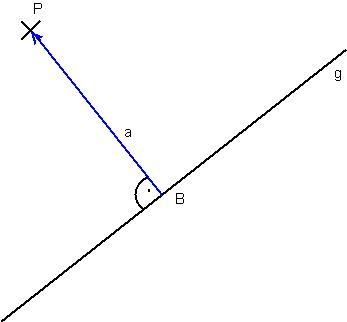
\includegraphics[scale=0.5]{abbildungen/lotfusspunkt.jpeg}
\end{figure}
\end{center}
Das Lotfu�punkt-Verfahren wird verwendet, um den Abstand eines Punktes von einer Geraden zu bestimmen.\\

Sei $g: \vec{x} = \vec{z} + \lambda \vec{u}$; $\lambda \in \mathbb{R}$ eine Gerade im $\mathbb{R}^3$ und $P$ ein Punkt.\\

\textbf{Definition:} Als \emph{Abstand} zwischen einem Punkt und einer Geraden bezeichnen wir die L�nge der k�rzesten Strecke zwischen den beiden.\\

Vektoriell gesehen bedeutet das, dass der Abstand des Punktes von der Geraden die L�nge desjenigen Vektors $\vec{a}$ ist, der senkrecht auf der Geraden steht und auf den Punkt $P$ zeigt.
Der Punkt $B$, an dem der Vektor senkrecht auf der Geraden steht wird \emph{Lotfu�punkt} von $P$ auf $g$ genannt.\\

Wir wissen:
\begin{align}
d(g, P) &= |\vec{a}|\\
&=|\vec{p}-\vec{b}| \label{GL2}
\end{align} 
Vom Vektor $\vec{b}$, dem Ortsvektor zum Punkt $B$, kennen wir folgende Eigenschaften:
\begin{align}
\vec{b} &\in g \\
(\vec{p} - \vec{b}) \cdot \vec{u} = 0 &\Leftrightarrow (\vec{p} - \vec{b}) \bot \vec{u} \label{Eig2}
\end{align}
Da $\vec{b} \in g$ k�nnen wir die Geradengleichung in \ref{Eig2} einsetzen:
\begin{align}
(\vec{p} - (\vec{z} + \lambda \vec{u})) \cdot \vec{u} &= 0 \label{GL5}
\end{align}
f�r ein bestimmtes $\lambda \in \mathbb{R}$\\
\ref{GL5} liefert eine Gleichung mit einer Unbekannten. L�st man diese Gleichung erh�lt man f�r $\lambda$:
\begin{align}
\lambda &= \frac{p_1 u_1 - z_1 u_1 + p_2 u_2 - z_2 u_2 + p_3 u_3 - z_3 u_3}{(u_1)^2 + (u_2)^2 + (u_3)^2}
\end{align}
Dies nachzurechnen sei dem Leser �berlassen. Im Folgenden verwenden wir der �bersichtlichkeit halber weiter $\lambda$.\\
Mithilfe dieses bestimmten $\lambda$ l�sst sich nun der Ortsvektor $\vec{b}$ und somit der Punkt $B$ bestimmen, womit das Problem auf eine Abstandsbestimmung zwischen zwei Punkten zur�ckgef�hrt wurde. Hierzu setzen wir das gerade errechnete $\lambda$ in die Geradengleichung ein.
\begin{align}
\vec{b} = \vec{z} + \lambda \vec{u}
\end{align}
Nach \ref{GL2} gilt nun:
\begin{align*}
d(g, P) &= |\vec{p} - \vec{z} -\lambda \vec{u}|\\
&=\sqrt{(p_1 -z_1 -\lambda u_1)^2 + (p_2 - z_2 -\lambda u_2)^2 + (p_3 -z_3 -\lambda u_3)^2}
\end{align*} \\
womit der gesuchte Abstand durch Einsetzen der gegebenen Komponenten und Berechnung des Betrages zu berechnen ist.\\

\section{Ebenen in vektorieller Darstellung}
Eine Ebene wird definiert durch einen \textbf{St�tzvektor} ($\vec{a})$ und zwei linear unabh�ngige \textbf{Spannvektoren} ($\vec{u}$ und $\vec{v}$).
\[ E: \vec{x} = \vec{a} + \lambda \vec{u} + \mu \vec{v}; \lambda, \mu \in \mathbb{R} \]

\textbf{Was leistet die vektorielle Darstellung einer Ebene?}\\
\begin{itemize}
	\item Punkttest
	\item Parameterfreie Darstellung
	\item Achsenschnittpunkte einer Ebene
	\item Lagebeziehungen
\end{itemize}

\section{Spurgeraden und Spurpunkte}
\label {spur}
\begin{definition}[Spurgeraden und Spurpunkte] Die drei Geraden, die durch die drei Schnittpunkte einer Ebene mit den kartesischen Achsen definiert sind, nennt man Spurgeraden.\\
Die Schnittpunkte einer Geraden mit den kartesischen Ebenen nennt man Spurpunkte.
\end{definition}

\section{Lagebeziehungen Ebene - Gerade im Raum}
M�gliche Lagebeziehungen zwischen einer Ebene und einer Geraden im $\mathbb{R}^3$: \\
\begin{enumerate}
	\item $E \cap g = \{ \} \Leftrightarrow E || g$
	\item $E \cap g = \{ S \}$
	\item $E \cap g = g \Leftrightarrow g \subset E$
\end{enumerate}

L�sung: Parameterform der Geraden und Parameterform der Ebene gleichsetzen.\\
M�gliche F�lle:\\
\begin{enumerate}
	\item keine L�sung $\Leftrightarrow E || g$
	\item eine eindeutige L�sung $\Leftrightarrow E \cap g = \{ S \}$
	\item unendlich viele L�sungen $\Leftrightarrow E \cap g = g$
\end{enumerate}

\section{Lagebeziehungen Ebene - Ebene im Raum (ohne NF)}
M�gliche Lagebeziehungen zwischen zwei Ebenen im $\mathbb{R}^3$: \\
\begin{enumerate}
	\item $E_1 \cap E_2 = \{ \} \Leftrightarrow E_1 || E_2$
	\item $E_1 \cap E_2 = g_s$
	\item $ E_1 \cap E_2 = E_1 = E_2 \Leftrightarrow E_1 \equiv E_2$ 
\end{enumerate}

L�sung: Parameterform beider Ebenen gleichsetzen.\\
M�gliche F�lle:\\
\begin{enumerate}
	\item keine L�sung $\Leftrightarrow E || g$
	\item unendlich viele L�sungen mit einem Parameter $\Leftrightarrow E_1 \cap E_2 = g_s$
	\item unendlich viele L�sungen mit zwei Parametern $E_1 \equiv E_2$
\end{enumerate}

%\section{Herleitung der Normalenform an einem Beispiel}
%\begin{bsp}
%Sei $\vec{x} = \left( \begin{array}{c} 1 \\ 1 \\ 2 \end{array} \right) + \lambda \left( \begin{array}{c} 1 \\ 0 \\ -2 \end{array} \right) + \mu \left( \begin{array}{c} -1 \\ 1 \\ -2 \end{array} \right); \lambda, \mu \in \mathbb{R}$\\
%$\rightarrow 2x_1 + 4x_2 + 1x_3 = 8$\\
%Dies l�sst sich auch schreiben als $\left( \begin{array}{c} x_1 \\ x_2 \\ x_3 \end{array} \right) \cdot \left( \begin{array}{c} 2 \\ 4 \\ 1 \end{array} \right) = 8$ \\
%$\Leftrightarrow \left( \begin{array}{c} x_1 \\ x_2 \\ x_3 \end{array} \right) \cdot \left( \begin{array}{c} 2 \\ 4 \\ 1 \end{array} \right) -8 = 0$ \\
%$\Leftrightarrow \left( \begin{array}{c} x_1 \\ x_2 \\ x_3 \end{array} \right) \cdot \left( \begin{array}{c} 2 \\ 4 \\ 1 \end{array} \right) - \left( \begin{array}{c} 2 \\ 4 \\ 1 \end{array} \right) \cdot \left( \begin{array}{c} 0 \\ 2 \\ 0 \end{array} \right) = 0$ da $8 = \left( \begin{array}{c} 2 \\ 4 \\ 1 \end{array} \right) \cdot \left( \begin{array}{c} 0 \\ 2 \\ 0 \end{array} \right)$\\
%$\Leftrightarrow \left[ \left( \begin{array}{c} x_1 \\ x_2 \\ x_3 \end{array} \right) - \left( \begin{array}{c} 0 \\ 2 \\ 0 \end{array} \right) \right] \cdot \left( \begin{array}{c} 2 \\ 4 \\ 1 \end{array} \right) = 0$\\

%$\vec{n} = \left( \begin{array}{c} 2 \\ 4 \\ 1 \end{array} \right) \bot E$ hei�t \textbf{Normalenvektor}.
%\end{bsp}

\section{Darstellungsm�glichkeiten von Ebenen}
\begin{enumerate}
	\item Parameterform (PF; Vektorgleichung) \\
	$E: \vec{x} = \vec{a} + \lambda \vec{u} + \mu \vec{v}; \lambda, \mu \in \mathbb{R}$
	\item Koordinatenform (KF; Skalargleichung) \\
	$E: x_1 a_1 + x_2 a_2 + x_3 a_3 = k; k \in \mathbb{R}$ \\
	$\vec{n} = \left( \begin{array}{c} a_1 \\ a_2 \\ a_3 \end{array} \right)$ ist ein Normalenvektor!
	\item Normalenform (NF)\\
	$E: (\vec{x} - \vec{p}) \cdot \vec{n} = 0 \Leftrightarrow \vec{x} \cdot \vec{n} = \vec{p} \cdot \vec{n}$\\
	dabei gilt:\\
	$\vec{p}$ Ortsvektor zu St�tzpunkt $P \in E$\\
	$\vec{x} - \vec{p} \in E$\\
	$\vec{n} \bot E$ Normalenvektor \\
	$\vec{n} \bot \vec{u} \land \vec{n} \bot \vec{v}$
\end{enumerate}

\subsection{Umwandlung von einer Ebenendarstellung in eine andere}
\begin{enumerate}
	\item $NF \rightarrow KF$\\
	NF ausmultiplizieren und man erh�lt eine KF
	\item $KF \rightarrow NF$\\
	$\vec{n} = \left( \begin{array}{c} a_1 \\ a_2 \\ a_3 \end{array} \right)$, als St�tzpunkt w�hle einen beliebigen Punkt $P \in E$, zum Beispiel durch \textit{raten} einer L�sung der Gleichung aus der Koordinatenform!\\
	 Einsetzen in $(\vec{x} - \vec{p}) \cdot \vec{n} = 0$
	 \item $PF \rightarrow NF$\\
	 $\vec{n}$ bestimmen mit $\vec{n} \cdot \vec{u} = 0 \land \vec{n} \cdot \vec{v} = 0$. Man erh�lt ein unterbestimmtes LGS, w�hlt eine Variable frei und erh�lt daraus die beiden anderen, also den Normalenvektor. Als N�chstes w�hlt man einen St�tzvektor $\vec{p} \in E$, der Einfachheit halber denselben St�tzvektor wie in der PF.
	 \item $NF \rightarrow PF$\\
	St�tzvektor �bernehmen. Finde dann zwei linear unabh�ngige Vektoren, die senkrecht auf dem Normalenvektor stehen. Dazu jeweils: Setze eine Koordinates des Normalenvektors $=0$, vertausche die beiden anderen und �ndere bei einer dieser beiden das Vorzeichen!
\end{enumerate}

\section{Lagebeziehungen zweier Ebenen im Raum (mit NF)}
\[E_1: \vec{x} \cdot \vec{n} = k_1 \]
\[E_2: \vec{x} \cdot \vec{m} = k_2 \]
\begin{enumerate}
	\item $E_1 || E_2 \Leftrightarrow \vec{n} = \lambda \vec{m}$
	\item $E_1 \equiv E_2 \Leftrightarrow \vec{n} = \lambda \vec{m} \land k_1 = \lambda k_2$
	\item $E_1 \cap E_2 = g \Leftrightarrow \vec{n} \neq \lambda \vec{m}$\\
	Spezialfall: $E_1 \bot E_2 \Leftrightarrow \vec{n} \cdot \vec{m} = 0$
\end{enumerate}

\section{Abstandsbestimmung (Zusammenfassung)}
P, Q, R Punkte; E, F Ebenen; g, h Geraden
\begin{itemize}
	\item $d(P, Q) = |\vec{p} - \vec{q}| = \sqrt{(p_1 - q_1)^2 + (p_2 - q_2)^2 + (p_3 - q_3)^2}$
	\item $d(P, g)$ Lotfu�punkt-Verfahren (siehe \ref{lotfusspunkt}) $\rightarrow$ Fl�chenberechnung
	\item $d(g, h)$ f�r $g \| h$:\\
	W�hle eine Gerade aus und berechne dann den Abstand dieser Gerade zum St�tzpunkt der anderen Geraden.
	\item $d(E, R)$\\
	\begin{definition} Unter dem Abstand eines Punktes von einer Ebene versteht man die k�rzeste Entfernung des Punktes zur Ebene. Diese ist die L�nge des Lotes vom Punkt auf die Ebene.\end{definition}
	\textbf{Verfahren 1:}\\
	gegeben: 
		\begin{align*}
		&E: x_1 + 8x_2 - 4x_3 = 25\\
		&R(2/0/1)
		\end{align*}
		\begin{enumerate}
			\item Bestimmung einer Lotgeraden $g_\bot$ zu $E$:\\
				\begin{align*}
				g_\bot: \vec{x} = \left( \begin{array}{c} 2 \\ 0 \\ 1 \end{array} \right) + \lambda \left( \begin{array}{c} 1 \\ 8 \\ -4 \end{array} \right); \lambda \in \mathbb{R}
				\end{align*}
			\item Bestimmung des Lotfu�punktes $F$ als gemeinsamer Punkt von $g_\bot$ und $E$.
				\begin{align*}
				x_1 &=2 + \lambda \\
				x_2 &=0 + 8\lambda \\
				x_3 &=1-4\lambda
				\end{align*}
				Einsetzen in die Ebenengleichung:
				\begin{align*}
				2 + \lambda + 8 \cdot (0 + 8\lambda) - 4 \cdot (1 - 4\lambda) &= 25 \\
				\Leftrightarrow \lambda &= \frac{1}{3}
				\end{align*}
				Einsetzen in die Koordinatengleichungen:
				\[F: \vec{f} =  \left( \begin{array}{c} \frac{7}{3} \\ \frac{8}{3} \\ -\frac{1}{3} \end{array} \right) \]
				\item \begin{align*}
				d(F, R) &= \sqrt{(2- \frac{7}{3})^2 + (0 - \frac{8}{3})^2 + (1+ \frac{1}{3})^2} \\
				&= 3
				\end{align*}
		\end{enumerate}
		\textbf{Verfahren 2 (LK):} \\
		Sei P der St�tzvektor der Ebene, $\vec{n_0}$ der normierte Normalenvektor an diesem Punkt, $\gamma$ der Winkel zwischen $\vec{n_0}$ und $\vec{PR}$ und $d$ der Abstandes des Punktes $R$ von der Ebene.
		$\vec{n_0}$ normierter Normalenvektor ($\vec{n_0} = \frac{\vec{n}}{|\vec{n}|}$) \\
		Sei $E: (\vec{x} - \vec{p}) \cdot \vec{n} = 0$ eine Ebene. Dann hei�t
		\[ E: (\vec{x} - \vec{p}) \cdot \vec{n_0} = 0 \]
		\textbf{Hesse'sche Normalenform} der Ebene.
		\begin{align*}
		\vec{n_0} \cdot \vec{PR} &= |\vec{n_0}| \cdot |\vec{PR}| \cdot \cos(\gamma) \\
		\cos(\gamma) &= \frac{d}{|\vec{PR}|} \\
		\Rightarrow \vec{n_0} \cdot \vec{PR} &= |\vec{n_0}| \cdot |\vec{PR}| \cdot \frac{d}{|\vec{PR}|} \\
		&= \vec{n_0} \cdot d \\
		&= d		\\
		\Leftrightarrow |\vec{n_0} \cdot (\vec{r} - \vec{p})| &= d
		\end{align*}
\item $d(E, g)$
\begin{enumerate}
	\item	$E \| g$
	\item HNF oder NF bestimmen
	\item Abstand berechnen.
\end{enumerate}
	\textbf{Merksatz:} Sind eine Gerade $g$ und eine Ebene $E$ zueinander parallel haben alle Punkte auf $g$ den selben Abstand zur Ebene. Wir berechnen den Abstand mithilfe von Verfahren 1 oder 2.
\item $d(E, F)$
\begin{enumerate}
	\item HNF oder NF aufstellen
	\item zeige $E \| F$
	\item W�hle einen beliebigen Punkt der Ebene $E$ und bestimme seinen Abstand zu $F$ (oder umgekehrt).
\end{enumerate}
\textbf{Beispielaufgabe (LK):} Bestimme alle Punkte, die zu 
\[ E: 4x_1 + 12x_2 - 3x_3 = 8 \]
den Abstand 2 haben. \\

\textbf{L�sungsstrategie:}
\begin{enumerate}
	\item Die gesuchten Punkte liegen auf zwei Ebenen, die zu $E$ den Abstand 2 haben.
	\item W�hle $P(p_1; p_2; p_3)$
	\item HNF von E aufstellen
	\item L�se Gleichung $d(E, P) = 2$ nach $p_1, p_2, p_3$ auf
	\item wegen der Betragsstriche ergeben sich zwei F�lle
	\item Stelle zwei Ebenen $E_1$ und $E_2$ auf, wobei $P$ und $P'$ Punkte der Ebenen sind. Den Normalenvektor �bernehmen wir von $E$
\end{enumerate}
\end{itemize}

\section{Abstand zweier windschiefer Geraden (LK)}
\textbf{Verfahren 1:}
\begin{itemize}
	\item $g_1$, $g_2$ haben keinen Schnittpunkt und sind nicht parallel. Sie sind also windschief.
	\item Stelle eine Hilfsebene auf, f�r die gilt:
	\begin{align*}
		E \| g_1 &\land g_2 \in E\\
		g_1 : \vec{x} &= \vec{u} + \lambda \vec{v}\\
		g_2 : \vec{x} &= \vec{w} + \mu \vec{r}\\
		E: \vec{x} &= \vec{w} + \mu \vec{r} + \lambda \vec{v}
	\end{align*}
	\item Forme $E$ in HNF um
	\item Berechne $d(E, g_1) = d(E, U)$
\end{itemize}
\textbf{Verfahren 2:}\\
Zu $g_1$ und $g_2$ gibt es zwei parallele Ebenen.
\begin{align*}
E_{g_1} &: (\vec{x} - \vec{u}) \cdot \vec{n} = 0 \\
E_{g_2} &: (\vec{x} - \vec{w}) \cdot \vec{n} = 0 \\
d &= | (\vec{u} - \vec{w}) \cdot \vec{n}_0 | \\
\vec{n} \bot \vec{v} &\land \vec{n} \bot \vec{r}
\end{align*}

\section{Schnittwinkel}
\textbf{Achtung}: Bei Berechnung von Winkeln sollte der Taschenrechner auf das Gradma� (\textit{D} oder \textit{Deg}) gestellt werden!\\s
\textbf{Vektor-Vektor:}\\
\begin{align*}
\cos \alpha = \frac{\vec{a} \cdot \vec{b}}{|\vec{a}| \cdot |\vec{b}|}
\end{align*}
\textbf{Gerade-Gerade:}\\
\begin{align*}
g: \vec{x} &= \vec{p} + \lambda \vec{u}\\
h: \vec{x} &= \vec{q} + \mu \vec{v} \\
& \lambda, \mu \in \mathbb{R}
\end{align*}
Schneiden sich zwei Geraden $g$ und $h$, so entstehen vier Winkel, zwei der Gr��e $\alpha$ und zwei der Gr��e $ \beta$. Der Schnittwinkel von $g$ und $h$ ist derjenige, der kleiner oder gleich $90^{\circ}$ ist. Es gilt also wiederum:
\begin{align*}
\cos \alpha = \frac{\vec{a} \cdot \vec{b}}{|\vec{a}| \cdot |\vec{b}|}
\end{align*}
\textbf{Ebene-Ebene:}\\
\begin{align*}
E_1: (\vec{x} - \vec{p}) \cdot \vec{n_1} = 0 \\
E_2: (\vec{x} - \vec{q}) \cdot \vec{n_2} = 0 
\end{align*}
Dann ist der Schnittwinkel zu errechnen durch
\begin{align*}
\cos \alpha = \frac{\vec{n_1} \cdot \vec{n_2}}{|\vec{n_1}| \cdot |\vec{n_2}|}
\end{align*}
\textbf{Merksatz}: Der Winkel zwischen den Ebenen ist gleich dem Winkel zwischen den Normalenvektoren!\\
\textbf{Gerade-Ebene:}\\
\begin{align*}
g: \vec{x} &= \vec{p} + \lambda \vec{u}\\
E_1: (\vec{x} - \vec{p}) \cdot \vec{n_1} = 0 \\
\lambda \in \mathbb{R}
\end{align*}
wegen $\cos (90^\circ - \alpha) = \sin {\alpha}$ folgt
\begin{align*}
\sin{\alpha} =\frac{\vec{n_1} \cdot \vec{u}}{|\vec{n_1}| \cdot |\vec{u}|}
\end{align*}

\section{Das Vektorprodukt (LK)}
\begin{definition}[Vektorprodukt]
F�r $\vec{a},\vec{b} \in \mathbb{R}^3$ definieren wir das Vektorprodukt als
\[ \vec{a} \times \vec{b} := \begin{pmatrix} \det \begin{pmatrix} a_2 & b_2 \\ a_3 & b_3 \end{pmatrix} \\ - \det \begin{pmatrix} a_1 & b_1 \\ a_3 & b_3 \end{pmatrix} \\ \det \begin{pmatrix} a_1 & b_2 \\ a_2 & b_2 \end{pmatrix} \end{pmatrix} \]\\
Der Betrag des Vektorprodukts entspricht dem Fl�cheninhalt des von den beiden Vektoren aufgespannten Parallelograms.
\end{definition}
\textbf{Eigenschaften des Vektorprodukts:}
\begin{enumerate}
\item $\vec{a} \times \vec{b} \perp \vec{a}, \vec{b} \Leftrightarrow \vec{a}, \vec{b}$ linear unabh�ngig
\item $\vec{a} \times \vec{b} = \vec{0} \Leftrightarrow \vec{a},\vec{b}$ linear abh�ngig
\item $\vec{a}, \vec{b}, \vec{a} \times \vec{b}$ bilden ein Rechtssystem
\item $\vec{a} \times \vec{b} = - \left( \vec{b} \times \vec{a} \right)$
\item $\vec{a} \times \left( \vec{b} + \vec{c} \right) = \vec{a} \times \vec{b} + \vec{a} \times \vec{c}$
\item $\vec{a} \times \left(r\vec{b} \right) = r \left(\vec{a} \times \vec{b} \right)$
\item $ \vec{a} \cdot \left( \vec{b} \times \vec{c} \right) = \left(\vec{a} \times \vec{b} \right) \cdot \vec{c}$
\item $\left(\vec{a} \times \vec{b}\right) \cdot \vec{a} = 0\\
\left(\vec{a} \times \vec{b} \right) \cdot \vec{b} = 0$
\item $\vec{d} = \vec{c} + r\vec{a} + s\vec{Ub} \Rightarrow \left(\vec{a} \times \vec{b}\right)\cdot \vec{c} = \left(\vec{a} \times \vec{b}\right) \cdot \vec{d}$
\end{enumerate}
\textbf{Volumen eines Spats:} 
\[ V = A \cdot h = \left| \left( \vec{a} \times \vec{b} \right) \cdot \vec{c} \right| \]

\chapter{Matrizen und Abbildungen}
\label{chmatrabb}
\begin{align*}
\begin{pmatrix}
a_{11} & a_{12} & \cdots & a_{1n} \\
a_{21} & a_{22} & \cdots & a_{2n} \\
\vdots & & & \vdots \\
a_{m1} & a_{m2} & \cdots & a_{mn}
\end{pmatrix}
\end{align*}
$m, n \in \mathbb{N}$\\

\begin{definition}[Matrix] Eine \textbf{Matrix} ist ein Zahlenschema mit m Zeilen und n Spalten.\\
$a_{ij}$ sind die Eintr�ge der Matrix aus $\mathbb{R}$, wobei $i = 1, \ldots, m$ und $j = 1, \ldots, n$.\\
Ist $A$ eine mxn-Matrix, so sagen wir $A \in \mathbb{R}^{mxn}$. mxn nennen wir auch den \textbf{Typ} oder die \textbf{Form} der Matrix.
\end{definition}

\begin{definition}[Quadratische Matrix] Eine Matrix hei�t \textbf{quadratisch}, wenn sie gleich viele Zeilen wie Spalten hat.
\end{definition}

\section{Rechnen mit Matrizen}
Wir stellen zun�chst fest: Jeder Vektor (so wie wir bisher Vektoren kennen) ist auch eine Matrix.\\
\begin{bsp}
$\vec{v} = \begin{pmatrix} 1 \\ 2 \\ 4 \end{pmatrix}$ ist eine 3x1-Matrix.
\end{bsp}

Andersherum besteht jede Matrix aus einem oder mehreren Spalten- bzw. Zeilenvektoren.\\
\begin{bsp}
$A = \begin{pmatrix} 1 & 2 & 3 & 4 \\ 5 & 6 & 7 & 8 \end{pmatrix}$ besteht aus den \textbf{Zeilenvektoren} $\begin{pmatrix} 1 & 2 & 3 & 4 \end{pmatrix}$ und $\begin{pmatrix} 5 & 6 & 7 & 8 \end{pmatrix}$, bzw. aus den \textbf{Spaltenvektoren} $\begin{pmatrix} 1 \\ 5 \end{pmatrix}$, $\begin{pmatrix} 2 \\ 6 \end{pmatrix}$, $\begin{pmatrix} 3 \\ 7 \end{pmatrix}$ und $\begin{pmatrix} 4 \\ 8 \end{pmatrix}$
\end{bsp}

\subsection{Multiplikation von Matrizen mit einem Skalar}
\textbf{Regel:} Eine Matrix $A$ wird mit einem Skalar multipliziert, indem man jedes einzelne Element mit dem Skalar multipliziert. 

\subsection{Addition von Matrizen}
\label{matradd}
\textbf{Regel:} Zwei Matrizen $A$ und $B$ vom selben Typ werden addiert, indem wir die entsprechenden Elemente addieren.\\

\begin{definition}[Nullmatrix] Die Matrix $0 = \begin{pmatrix} 0 & \cdots & 0 \\ \vdots & \ddots & \vdots \\ 0 & \cdots & 0 \end{pmatrix}$ mit $a_{ij} = 0$ f�r alle i,j hei�t \textbf{Nullmatrix}.
\end{definition}
Es gilt: $A + 0 = 0 + A = A$ wenn $A$ und $0$ vom selben Typ sind.\\
\textbf{Achtung:} Im Folgenden wird f�r die Zahl Null und die Nullmatrix das gleiche Symbol "`0"' verwendet!


\subsection{Multiplikation von Matrizen}
\label{matrmulti}
\textbf{Regel:} $A \in \mathbb{R}^{lxm}, B \in \mathbb{R}^{mxn}$\\
Das Produkt ist $AB = C \in \mathbb{R}^{lxn}$\\
Die Elemente $c_{ij}$ erh�lt man, indem man das Skalarprodukt des i-ten Zeilenvektors von $A$ mit dem j-ten Spaltenvektor von $B$ berechnet.\\
\begin{definition}[Einheitsmatrix] Die nxn Matrix $\begin{pmatrix} 1 & 0 & 0 & \cdots & 0 \\ 0 & 1 & 0 & \vdots & 0 \\ \vdots & & \ddots & 0 & \vdots \\ 0 & \cdots & 0 & 1 & 0 \\ 0 & \cdots & & 0 & 1 \end{pmatrix}$ mit den Eintr�gen $c_{ij} = \begin{cases} 1 & i = j \\ 0 & i \neq j\end{cases}$ hei�t \textbf{Einheitsmatrix}.
\end{definition}
\textbf{Achtung:} Das Produkt $AB$ ist nur definiert, wenn die Anzahl der Spalten von $A$ gleich der Anzahl der Zeilen von $B$ ist.\\

\subsection{Rechengesetze der Matrizenrechnung:}
Gegeben seien die Matrizen $A$, $B$ und $C$ vom jeweils passenden Typ.
\begin{itemize}
	\item Assoziativgesetz:\\
	$(AB) \cdot C = A \cdot (BC)$\\
	$(A+B) + C = A+ (B + C)$
	\item Distributivgesetze:\\
	$(A+B) \cdot C = AC + BC$\\
	$A \cdot (B+C) = AB + AC$
	\item $(\lambda A)(\mu B) = (\lambda \mu)(AB)$
	\item $A \cdot (\lambda B) = \lambda AB$
	\item $A \cdot E_n = E_n \cdot A = A \Rightarrow E_n$ ist das neutrale Element bzgl ($\cdot$)
	\item $A + 0 = 0 + A = A \Rightarrow 0$ ist das neutrale Element bzgl (+)
	\item Das Kommutativgesetz gilt bei der Multiplikation von Matrizen im Allgemeinen \textbf{nicht}!
\end{itemize}

\subsection{Determinante von 2x2-Matrizen}
\begin{definition}[Determinante] Die \textbf{Determinante} einer 2x2 Matrix $\begin{pmatrix} a & b \\ c & d \end{pmatrix}$ ist eine Zahl $\in \mathbb{R}$ gegeben durch $det(A) = ad - bc$
\end{definition}

\section{Affine Abbildungen in der Ebene}
\begin{definition}[Affine Abbildung] Eine \textbf{affine Abbildung} im $\mathbb{R}^2$ ist gegeben durch 
\begin{align*}
\alpha: \vec{x'} = A \cdot \vec{x} + b
\end{align*}
\end{definition}
$A$ ist eine 2x2-Matrix mit $det(A) \neq 0$ und $\vec{b}$ ist ein Vektor mit zwei Koordinaten. Diese Darstellung hei�t \textbf{Matrizendarstellung einer affinen Abbildung}. Andere Darstellungsm�glichkeiten sind die \textbf{Vektordarstellung einer affinen Abbildung}:
\begin{align*}
\alpha: \begin{pmatrix} x \\ y \end{pmatrix}' = \begin{pmatrix} a \\ c \end{pmatrix} \cdot x + \begin{pmatrix} b \\ d \end{pmatrix} \cdot y + \begin{pmatrix} e \\ f \end{pmatrix}
\end{align*}
oder die \textbf{Koordinatendarstellung einer affinen Abbildung}
\begin{align*}
\alpha: \begin{array}{l} x' = ax + by+ e \\ y' = cx + dy + f \end{array}
\end{align*}
Bemerkung: Jede affine Abbildung ist durch $A$ und $\vec{b}$ festgelegt. Sie bildet den Punkt (x, y) mit dem Ortsvektor $\vec{x} = \begin{pmatrix} x \\ y \end{pmatrix}$ auf den Punkt (x', y') mit dem Ortsvektor $\vec{x'} = \begin{pmatrix} x' \\ y' \end{pmatrix}$ ab.\\
Feststellung: Jede affine Abbildung ist eindeutig festgelegt durch die Angabe von drei Urbildpunkten und drei zugeh�rigen Bildpunkten, solange diese nicht auf einer Geraden liegen.\\
\begin{definition} P hei�t \textbf{Urbildpunkt} und P \textbf{Bildpunkt}. \end{definition}

\textbf{Eigenschaften einer affinen Abbildung:}
\begin{enumerate}
	\item geradentreu, d.h. Geraden werden auf Geraden abgebildet
	\item parallelentreu, d.h. zueinander parallele Geraden werden auf zueinander parallele Geraden abgebildet
	\item umkehrbar, d.h. zu jedem Bildpunkt gibt es genau einen Urbildpunkt
	\item teilverh�ltnistreu
\end{enumerate}
\textbf{Folgerungen}:
\begin{enumerate}
	\item Dreiecke werden auf Dreiecke abgebildet
	\item Parallelogramme auf Parallelogramme
	\item Mittelpunkte von Strecken auf Mittelpunkte von Strecken
\end{enumerate}
\textbf{Eigenschaften, die affine Abbildungen haben k�nnen, aber nicht m�ssen:}
\begin{itemize}
	\item l�ngentreu (zu �berpr�fen an einer Zeichnung)
	\item winkeltreu (zu �berpr�fen an einer Zeichnung)
	\item fl�cheninhaltstreu $\Leftrightarrow |det(A)| = 1$
	\item orientierungstreu $\Leftrightarrow det(A) > 0$
	\item orientierungsumkehrend $\Leftrightarrow det(A) < 0$
	\item Fixpunkte haben, d.h. $P = P'$
	\item Fixpunktgeraden haben (Gerade, auf der nur Fixpunkte liegen $\rightarrow$ Spiegelung an dieser Geraden)
	\item Fixgeraden haben (eine Fixgerade ist eine Gerade, die wieder auf sich selbst abgebildet wird. Dabei k�nnen die einzelnen Punkte der Gerade aber untereinander vertauscht werden, es ist also keine Fix\textbf{punkt}gerade
\end{itemize}

\textbf{Spezielle affine Abbildungen:}
\begin{itemize}
	\item Drehung um $\vec{p}$ mit dem Winkel $\phi$ \\
		\begin{itemize}
			\item fl�cheninhaltstreu
			\item orientierungstreu 
			\item l�ngentreu
			\item winkeltreu
		\end{itemize}
		Allgemeine Form: 
		\begin{align*}
			\alpha: \vec{x'} = \begin{pmatrix} \cos{\phi} & - \sin{\phi} \\ \sin{\phi} & \cos{\phi} \end{pmatrix} \vec{x} + 2\vec{p}
		\end{align*}
	\item zentrische Streckung von einem Streckzentrum Z mit dem Streckfaktor k
		\begin{itemize}
			\item orientierungstreu
			\item winkeltreu
		\end{itemize}
		Allgemeine Form:
		\begin{align*}
			\alpha: \vec{x'} = \begin{pmatrix} k & 0 \\ 0 & k \end{pmatrix} \vec{x} + \vec{z}
		\end{align*}
		wobei $\vec{z}$ das Streckzentrum ist und $k$ der Streckfaktor.
	\item Spiegelung an einer Achse / Gerade
		\begin{itemize}
			\item fl�cheninhaltstreu
			\item orientierungsumkehrend
			\item l�ngentreu
			\item winkeltreu
		\end{itemize}
		Allgemeine Form einer Spiegelung an einer Ursprungsgeraden, die mit der x-Achse den Winkel $\phi$ einschlie�t:
		\begin{align*}
			\alpha: \vec{x'} = \begin{pmatrix} \cos{2\phi} & \sin{2\phi} \\ \sin{2\phi} & - \cos{2\phi} \end{pmatrix} \vec{x}
		\end{align*}
	\item Verschiebung um einen Vektor $\vec{v}$
		\begin{itemize}
			\item fl�cheninhaltstreu
			\item winkeltreu
			\item l�ngentreu
			\item orientierungstreu
		\end{itemize}
		Allgemeine Form:
		\begin{align*}
			\alpha: \vec{x'} = \begin{pmatrix} 1 & 0 \\ 0 & 1 \end{pmatrix} \vec{x} + \vec{v}
		\end{align*}
		wobei um den Vektor $\vec{v}$ verschoben wird.
	\item Scherung an einer Geraden $g$ mit dem Winkel $\phi$
		\begin{itemize}
			\item fl�cheninhaltstreu
			\item orientierungstreu
		\end{itemize}
		Scherung an der x-Achse mit Winkel $\phi$
		\begin{align*}
			\alpha: \vec{x'} = \begin{pmatrix} 1 & \tan{\phi} \\ 0 & 1 \end{pmatrix} \vec{x}
		\end{align*}
	\item Punktspiegelung \\
		siehe Drehung um einen Punkt (mit 180�)
\end{itemize}

\subsection{Affine Abbildungen rechnerisch bestimmen}
Gegeben sind drei Urbildpunkte und die entsprechenden Bildpunkte. \\
Eine affine Abbildung ist gegeben durch
\begin{align*}
\alpha: \vec{x'} = A\vec{x} + \vec{c} \Rightarrow \left| \begin{matrix} x' = a_{11} x + a_{12} y + c_1 \\ y' = a_{21} x + a_{22} y + c_2 \end{matrix} \right|
\end{align*}
Durch einsetzen der Urbild- bzw. der Bildpunkte erh�lt man zwei LGS mit je drei Gleichungen und drei Unbekannten, die man genau dann eindeutig l�sen kann, wenn die Abbildung affin ist.

\subsection{Bestimmung der Fixpunkte und Fixpunktgeraden}
Gegeben sei eine affine Abbildung durch $\alpha: \vec{x'} = A \vec{x} + \vec{c}$. \\
Ansatz: $\vec{x'} = \vec{x}$ \\
Zu l�sen ist also
\begin{align*}
	\begin{pmatrix} x \\ y \end{pmatrix} = A \begin{pmatrix} x \\ y \end{pmatrix}
\end{align*}
Bei einer eindeutigen L�sung gibt es einen Fixpunkt, gibt es unendlich viele L�sungen handelt es sich um eine Fixpunktgerade.

\subsection{Verketten von Abbildungen}
Zwei Abbildungen verketten hei�t, zwei Abbildungen hintereinander ausf�hren. $\beta \circ \alpha$ bedeutet, dass zuerst $\alpha$ ausgef�hrt wird, und danach $\beta$. \textbf{Achtung}: In der Regel gilt $\alpha \circ \beta \neq \beta \circ \alpha$!\\
Die neue Abbildungsmatrix der verketteten Abbildung lautet im Fall $\beta \circ \alpha$: $B \cdot A$ und im Fall $\alpha \circ \beta$: $A \cdot B$.\\
Eine Verkettung von zwei Abbildungen ist genau dann eine affine Abbildung, wenn auch die beiden Ausgangsabbildungen affine Abbildungen sind. Es gilt au�erdem:
\begin{satz}[Determinantensatz]
\[ \det(AB) = \det(A) \cdot \det(B) \]
\end{satz}

\subsection{Umkehrabbildungen}
\begin{definition}[Umkehrabbildung und inverse Matrix]
Wir definieren: $\alpha^{-1}$ \textbf{Umkehrabbildung} von $\alpha$ $\Leftrightarrow \alpha^{-1} \circ \alpha = \begin{pmatrix} 1 & 0 \\ 0 & 1 \end{pmatrix} = id$. Die zugeh�rige Umkehrmatrix hei�t \textbf{inverse Matrix} und wird mit $A^{-1}$ bezeichnet. Es gilt $A^{-1} \cdot A = A \cdot A^{-1}$
\end{definition}
\begin{satz}
Affine Abbildungen sind umkehrbar.
\end{satz}
Im Falle von 2x2 Matrizen kann man die inverse Matrix einer Matrix $A = \begin{pmatrix} a_1 & b_1 \\ a_2 & b_2 \end{pmatrix}$ mit der Formel
\[A^{-1} = \frac{1}{\det(A)} \begin{pmatrix} b_2 & - b_1 \\ -a_2 & a_1 \end{pmatrix}\]
berechnen.

\subsection{Affine Abbildungen und Fl�chen�nderung}
\begin{satz}
Sei $\det(A) = k$. Dann ist $|k|$ der Fl�chen�nderungsfaktor jeder affinen Abbildung $\alpha: \vec{x'} = A\vec{x} + \vec{c}$
\end{satz}

\subsection{Eigenwerte und Eigenvektoren, Fixgeraden}
\begin{definition}[Eigenwert]
Ein Skalar $\lambda$ hei�t \textbf{Eigenwert der Matrix A} wenn es mindestens einen Vektor $\vec{v}$ gibt, so dass gilt
\[A\vec{v} = \lambda\vec{v} \]
\end{definition}
\begin{satz}
Die Eigenwerte der Matrix A sind genau die L�sungen der Gleichung
\[ \det(A-\lambda E) = 0 \]
\end{satz}
Es schlie�t sich logischer Weise an
\begin{definition}[Eigenvektoren]
Ein Vektor $\vec{v}$ hei�t \textbf{Eigenvektor der Matrix A zum Eigenwert $\lambda$}, wenn gilt
\[A\vec{v} = \lambda\vec{v} \]
\end{definition}
\begin{satz}
Die Eigenvektoren sind genau die L�sungsvektoren von
\[ \det(A-\lambda E) \vec{v} = \vec{0} \]
\end{satz}
\begin{definition}[Fixgerade]
Eine Fixgerade ist eine Gerade, die durch eine Abbildung $\alpha$ auf sich selbst abgebildet wird. Es gilt also
\begin{align*}
P \in g \Rightarrow P' \in g
\end{align*}
\end{definition}
\textbf{Achtung}: Dies bedeutet nicht, dass jeder Punkt der Geraden auf sich selbst abgebildet werden muss. Wird jeder Punkt einer Geraden auf sich selbst abgebildet, nennt man diese Gerade Fixpunktgerade. Fixpunktgeraden sind Fixgeraden.\\
Sei $\alpha: \vec{x'} = A\vec{x} + \vec{c}$ eine affine Abbildung.\\
Hat die Abbildung einen oder mehrere Fixpunkte, so ist es einfach, die Fixgeraden zu bestimmen. Die Fixgeraden sind in diesen F�llen n�mlich genau die Geraden mit den Fixvektoren als St�tzvektoren und den Eigenvektoren der Matrix $A$ als Richtungsvektoren.\\
Deutlich komplizierter wird die Bestimmung der Fixgeraden, wenn die Abbildung keine Fixpunkte hat.\\
Ist $g: \vec{x} = \vec{p} + t \vec{u}$ eine Fixgerade, so muss gelten
\[ \vec{p'} = A\vec{p} + \vec{c} \wedge \vec{p'} = \vec{p} + t \vec{u} \]
Dies wiederum f�hrt uns zur so genannten \textbf{St�tzpunktgleichung}:
\[A\vec{p} - \vec{p} = t \vec{u} \]
Alle Vektoren $\vec{p}$, die diese Gleichung erf�llen, sind St�tzvektoren von Fixgeraden der Abbildung.

\subsection{Affine Abbildungen mit Fixpunkt 0}
$\alpha: \vec{x'} = A\vec{x}$\\
Wir unterscheiden drei F�lle:
\begin{enumerate}
\item $A$ besitzt zwei verschiedene Eigenwert $\lambda_1, \lambda_2$ $\Rightarrow \alpha$ ist i.A. eine Euleraffinit�t
\item $A$ besitzt einen Eigenwert $\lambda$ $\Rightarrow \alpha$ ist i.A. eine Streckscherung
\item $A$ besitzt keinen Eigenwert $\Rightarrow \alpha$ ist i.A. eine Affindrehung
\end{enumerate}
\begin{definition}[Euler-Affinit�t]
Eine affine Abbildung, die zwei Eigenwerte besitzt, nennt man \textbf{Euler-Affinit�t}.
\end{definition}
\begin{definition}
Eine affine Abbildung f�r die gilt
\begin{enumerate}
\item $P \in g_{2} \Rightarrow P = P'$
\item $P \in g_{2} \Rightarrow \vec{PP'} \parallel g_{1}$
\item $\vec{G_{2}P'} = \lambda_1 \vec{G_{2}P}$
\end{enumerate}
hei�t \textbf{Parallelstreckung} an der Streckachse $g_{2}$ parallel zu $g_{1}$ mit dem Streckfaktor $\lambda_1$
\end{definition}
\begin{satz}
Eine Euler-Affinit�t ist eine Linearkombination aus zwei Parallelstreckungen
\end{satz}

\section{Parallelprojektion}
\begin{definition}[Projektion]
Eine \textbf{Projektion} ist eine Abbildung des Raumes in eine Ebene (Projektionsebene). Die Gerade zwischen Punkt $P$ und dem Bildpunkt $P'$ der Projektion hei�t \textbf{Projektionsgerade}. Sind alle Projektionsgeraden parallel, so spricht man von einer \textbf{Parallelprojektion}.
\end{definition}
\begin{satz}
Die Abbildungsmatrix einer Parallelprojektion hat als Spalten die Ortsvektoren der Bildpunkte der Einheitsvektoren.
\end{satz}

Nun, wie berechnet man eine solche Projektionsmatrix ( = Abbildungsmatrix einer Projektion)? \\
Dies ist ganz einfach, denn nach obigem Satz muss man nur die Bildpunkte der Einheitsvektoren bestimmen. Dazu nimmt man den ersten Einheitsvektor als St�tzvektor einer Geraden $g$ und den Richtungsvektor der Projektionsgeraden als Richtungsvektor von $g$. Dann schneidet man die Gerade $g$ mit der Projektionsebene und erh�lt den Schnittpunkt $S$, der gleichzeitig der Bildpunkt $P'$ ist. Analog verf�hrt man mit dem zweiten und dritten Einheitsvektor, wonach man die Projektionsmatrix bestimmen kann.

\section{Prozessmatrizen und Bedarfsmatrizen}
Prozessmatrizen dienen dazu, den Verlauf eines Prozesses �ber mehrere Schritte zu bestimmen. Ein Spezialfall der Prozessmatrizen sind die Bedarfsmatrizen. Mit ihnen l�sst sich z.B. die Rohstoffmenge berechnen, die zur Herstellung von Produkten ben�tigt wird. Wir veranschaulichen dies an einem
\begin{bsp}
Seien $D_1, D_2$ zwei verschiedene D�nger und $R_1, R_2, R_3$ drei verschiedene Rohstoffe, die zur Herstellung dieser D�nger verwendet werden. Den Bedarf an Rohstoffen pro Kilogramm D�nger kann man folgender Tabelle entnehmen:\\
\begin{tabular}{c|c|c|c|}
 & $R_1 (y_1)$ & $R_2 (y_2)$ & $R_3 (y_3)$ \\
\hline
$D_1 (x_1)$ & 0.5 & 0.3 & 0.2\\
\hline
$D_2 (x_2)$ & 0.2 & 0.2 &0.4 \\
\end{tabular}\\
Aus dieser Tabelle l�sst sich das folgende LGS erstellen:
\begin{align*}
y_1= 0.5x_1 + 0.2x_2\\
y_2= 0.3 x_1 + 0.2x_2\\
y_3= 0.2x_1 + 0.4x_2
\end{align*}
Dieses LGS sieht in Matrizenschreibweise wiederum so aus:
\begin{align*}
\begin{pmatrix} y_1 \\ y_2 \\ y_3\end{pmatrix} = \underbrace{\begin{pmatrix} 0.5 & 0.2 \\ 0.3 & 0.2 \\ 0.2 & 0.4 \end{pmatrix}}_{\textrm{Bedarfsmatrix}} \cdot \begin{pmatrix} x_1 \\ x_2 \end{pmatrix}
\end{align*}
Mithilfe dieser Matrix l�sst sich nun also z.B. ausrechnen, wie viel Kilogramm von jedem Rohstoff zur Herstellung von je einer Tonne D�nger ben�tigt werden.
\end{bsp}

Prozessmatrizen funktionieren �hnlich wie die Bedarfsmatrizen, nur dass sie stattdessen einen Prozess beschreiben, zum Beispiel die Entwicklung einer Maik�ferpopulation �ber mehrere Monate. Als Beispiel sei die folgende Aufgabe genannt:
\begin{bsp}
Die Entwicklung einer weiblichen K�ferpopulation kann modellhaft wie folgt beschrieben werden: Ein Weibchen legt 20 Eier und stirb kurz darauf. Nach einem Monat entwickeln sich aus den Eiern Larven, von denen aber nur 30\% �berleben. Nach einem weiteren Monat verpuppen sich 40\% der Larven und werden zu weiblichen K�fern, die wieder 20 Eier legen.\\
\quad\\
Aus diesem Aufgabentext l�sst sich folgende Tabelle entnehmen:\\
\begin{tabular}{l|ccc}
nach / von & K & E & L\\
\hline
K & 0 & 0 & 2/5\\
E & 20 & 0 & 0\\
L & 0 &3/10 & 0
\end{tabular} \\
Aus dieser Tabelle wiederum folgt sofort folgende Matrix:
\[ A = \underbrace{\begin{pmatrix} 0 & 0 &\frac{2}{5}\\ 20 & 0 & 0 \\ 0 & \frac{3}{10} & 0 \end{pmatrix}}_{\textrm{Prozessmatrix}} \]
\end{bsp}
Multipliziert man die Matrix mit einem Ausgangsvektor, so erh�lt man die Verteilung nach einer Zeiteinheit. M�chte man die Verteilung nach $n$ Zeiteinheiten errechnen, muss man die Matrix $n$-mal mit dem Vektor multiplizieren, bzw. die Matrix $A^n$ mit dem Vektor multiplizieren.



%\part{Stochastik}

%\chapter{Beschreibung von Zufallsexperimenten}
%\input{zufallsexperimente.tex}



%\newpage
%\appendix
%\section{Lotfupunkt-Verfahren}
%\input{lotfusspunkt.tex}\label{anhangA}

\end{document}